\documentclass[final,leqno,onefignum,onetabnum]{siamltex1213bueler}
% siamltex1213bueler.cls is a two or three line change of siamltex1213.cls to permit
% pdflatex to work and not spew warnings

\usepackage{amssymb,amsmath}

\usepackage{times}

\usepackage{tikz}

\newtheorem{example}{Example}

% math macros
\newcommand\bb{\mathbf{b}}
\newcommand\bbf{\mathbf{f}}
\newcommand\bG{\mathbf{G}}
\newcommand\bn{\mathbf{n}}
\newcommand\bq{\mathbf{q}}
\newcommand\br{\mathbf{r}}
\newcommand\bu{\mathbf{u}}
\newcommand\bv{\mathbf{v}}
\newcommand\bx{\mathbf{x}}
\newcommand\by{\mathbf{y}}

\newcommand\bQ{\mathbf{Q}}
\newcommand\bV{\mathbf{V}}
\newcommand\bX{\mathbf{X}}
\newcommand\bY{\mathbf{Y}}

\newcommand\CC{\mathbb{C}}
\newcommand{\DDt}[1]{\ensuremath{\frac{d #1}{d t}}}
\newcommand{\ddt}[1]{\ensuremath{\frac{\partial #1}{\partial t}}}
\newcommand{\ddx}[1]{\ensuremath{\frac{\partial #1}{\partial x}}}
\newcommand{\ddy}[1]{\ensuremath{\frac{\partial #1}{\partial y}}}
\newcommand{\ddxp}[1]{\ensuremath{\frac{\partial #1}{\partial x'}}}
\newcommand{\ddz}[1]{\ensuremath{\frac{\partial #1}{\partial z}}}
\newcommand{\ddxx}[1]{\ensuremath{\frac{\partial^2 #1}{\partial x^2}}}
\newcommand{\ddyy}[1]{\ensuremath{\frac{\partial^2 #1}{\partial y^2}}}
\newcommand{\ddxy}[1]{\ensuremath{\frac{\partial^2 #1}{\partial x \partial y}}}
\newcommand{\ddzz}[1]{\ensuremath{\frac{\partial^2 #1}{\partial z^2}}}
\newcommand{\Div}{\nabla\cdot}
\newcommand\eps{\epsilon}
\renewcommand{\grad}{\nabla}
\newcommand{\ihat}{\mathbf{i}}
\newcommand{\ip}[2]{\ensuremath{\left<#1,#2\right>}}
\newcommand{\jhat}{\mathbf{j}}
\newcommand{\khat}{\mathbf{k}}
\newcommand{\nhat}{\mathbf{n}}
\newcommand\lam{\lambda}
\newcommand\lap{\triangle}
\newcommand\Matlab{\textsc{Matlab}\xspace}
\newcommand\RR{\mathbb{R}}
\newcommand\vf{\varphi}



\title{Conservation for fluid layers with free boundaries\thanks{Draft date: \today.  Supported by NASA grant \# NNX13AM16G.}} 

\author{Ed Bueler\thanks{Dept.~of Mathematics and Statistics, University of Alaska Fairbanks (\texttt{elbueler@alaska.edu}).}}

\begin{document}
\maketitle
\slugger{siap}{xxxx}{xx}{x}{x--x}

\begin{abstract}
FIXME
\end{abstract}


\pagestyle{myheadings}
\thispagestyle{plain}
\markboth{ED BUELER}{CONSERVATION FOR FLUID LAYERS WITH FREE-BOUNDARIES}


\section{Introduction}  \label{sec:intro}

Consider a fluid which moves in a thin layer, on some fixed substrate, in which fluid mass can be added or removed from the layer by external agents.  Through flow and these addition (accumulation, precipitation, \dots) and removal (ablation, evaporation, \dots) processes, the thickness of the layer can change in time.  The balance between flow and these processes also determines the extent of the fluid-covered area, and, for example, sufficient ablation can remove the fluid entirely.

We consider those models of such fluid layers in which the fluid geometry is fully described by a nonnegative thickness function.  In such models the addition/removal processes are combined into a signed source term in a two-spatial-dimension conservation equation which applies to those areas where the thickness is positive.  The addition/removal processes are necessarily assumed to be defined on a larger fixed region of the substrate.  The region of positive thickness, i.e.~the fluid-covered domain, changes in time, and thus the problem is of free-boundary type.  The conservation equation, plus further models for how the layer geometry and flow are related, combine with the models determining the addition/removal processes to determine the location of the free/moving boundary where the thickness goes to zero.

Problems of this type appear within climate and forecasting models, especially for the ice sheet, sea ice, and ocean components of the earth system (Figure \ref{fig:climatepictures}).  Though these geoscientific applications drive the author's interest in the problem, the situation is also as familiar as the build-up and drying of rain on a car windshield, the making of pancakes, and so on.

\begin{figure}[ht]
\begin{center}
FIGURE (FIXME)
%\includegraphics[width=2.0in,keepaspectratio=true]{}
\end{center}
\caption{Free-boundary fluid layer mass conservation problems occur for several components of the earth-system and climate models, including ice sheet (a), sea ice (b), and ocean (c) components.}
\label{fig:climatepictures}
\end{figure}

In the climate modeling context, determining the fluid-covered area is a leading-order modeling goal.  In the icy cases above, for example, snow and ice are much more reflective of sunlight than the substrate they cover (i.e.~land and ocean, respectively, for ice sheets and sea ice), so deciding whether areas are ice-covered or ice-free is a significant part of the state of a coupled earth-system model.  Simultaneously, however, conservation of mass, including accurate accounting of mass transfers to and from the modeled fluid to other earth system components, is a major modeling goal.  This paper mathematically analyzes the well-posedness of, and tradeoffs inherent in, models of such fluid layers as they are influenced by their climate.

If the fluid is modeled as having constant density then the nonnegative thickness is the conserved quantity, equivalent to mass per unit area of the substrate.  In models for variable density fluids the vertical integral of density is the conserved quantity in the two-dimensional form of the problem, and again it must be nonnegative.  However, we consider only conservation of nonnegative scalar properties, and not, for example conservation of vectors like momentum.  As mass conservation of constant-density fluids is the primary example, for simplicity we call the conserved quantity ``mass'' and the corresponding nonnegative variable ``thickness''.

To be precise, suppose $\Omega \subset \RR^d$, $d\ge 1$, is a bounded open region with regular (Lipshitz) boundary.  Let $T>0$.  The layer thickness function $u(x,t)$ is defined for all $x\in \bar\Omega$ and $t \in [0,T]$, but where there is no fluid we have $u(x,t)=0$.  The time-dependent models we consider are usually stated in \emph{strong form}, in which case they include both a mass conservation equation and a sometimes-unstated constraint:
\begin{align}
u_t + \Div \bq &= f(u,x,t) &&\text{in } \Omega \times (0,T), \text{ where } u > 0 \label{eq:massconserve} \\
u &\ge 0 &&\text{in } \bar\Omega \times [0,T]. \label{eq:constraint}
\end{align}
Conservation equation \eqref{eq:massconserve} only applies where the layer \emph{exists} ($u>0$) and not in any open set on which it is \emph{absent} ($u=0$).  Constraint \eqref{eq:constraint} simply comes from the meaning of $u$ as a thickness.

The above equations are assumed to be parts of the model, but of course they are not yet a complete model.  Well-posedness of any model including \eqref{eq:massconserve} and \eqref{eq:constraint} requires additional information about $\bq$ and $f$ (next), but it also requires precise specification of admissible functions and a weak formulation, which we address in Sections \ref{sec:weakform} and \ref{sec:wellposed}.

The primary form of the flux $\bq$ considered here is local but reasonably general,
\begin{equation}
\bq = \bq(\grad u,u,x,t). \label{eq:fluxdepends}
\end{equation}
Flux assumptions which apply for most of the examples in the paper are given in Subsection \ref{subsec:fluxassumptions}.  In some examples the process is diffusive, and could be written in the form $\bq=- D \grad u + (\text{other terms})$, where $D > 0$ has various dependence on $t,x,u,|\grad u|$; see subsections \ref{subsec:plap} and \ref{subsec:powertransform}.

In advective-flux examples covered by \eqref{eq:fluxdepends} we think of the fluid moving at some (vertically-averaged) velocity $\bX=\bX(x,t)$ determined by external factors, and thus $\bq = \bX u$ (subsection \ref{subsec:advect}).  Many of our results for such advective fluxes apply even if $\bX$ comes from a (coupled) solution of a momentum conservation system, as long as it has the regularity we need to apply the theory (subsection \ref{subsec:fluxassumptions}).  In any case, we consider models where $\bq$ depends \emph{globally} on the conserved quantity $u$ and its derivatives, through integrals over $\Omega$, in subsection \ref{subsec:nonlocal}.

The ideas and results in this paper are of most interest if the \emph{source function} $f(u,x,t)$ in \eqref{eq:massconserve} takes either sign.  If $f\ge 0$ everywhere and if the initial state is also nonnegative ($u(x,0)\ge 0$) then active enforcement of constraint \eqref{eq:constraint} may not be necessary.  In that case the existence of a maximum principle for the discretized problem (semi- or fully-discretized) will imply the nonnegativity of the solution $u(x,t)$.  By contrast, $f<0$ models the removal of fluid, in some cases sending the thickness $u$ to zero.  Active enforcement of \eqref{eq:constraint} then generates a free boundary, the location of which comes from the combined solution of \eqref{eq:massconserve} and \eqref{eq:constraint}, along with a particular functional form of the flux $\bq$.

The source term $f(u,x,t)$ is allowed to be nonlinear in $u$ because positive or negative feedback between layer thickness $u$ and the source $f$ occurs in certain applications (e.g.~for glaciers \cite{Jouvetetal2011}).  However, our results say nothing new about such cases.  Indeed, when proving well-posedness of time-steps in section \ref{sec:wellposed} we simplify to the $u$-independent case $f=f(x,t)$.

Numerical approximations of these time-evolving fluid layer problems necessarily discretize time in some manner, and our analysis is based on this fact.  We semi-discretize the mass conservation equation in time by a one-step method and pose the single-time-step, continuous-space problem in weak variational form  (section \ref{sec:weakform}).  Sections \ref{sec:timeseries} and \ref{sec:wellposed} address the discretized-time problem independently of spatial discretization.  By contrast, section \ref{sec:spacediscretized} extends our results to a fully-discretized, unstructured finite volume element method framework \cite{Cai1990}.

Given a time-discretization, each time-step requires the solution of a (continuous) free-boundary problem in space.  An immediate question is:
  \begin{quote}
  \renewcommand{\labelenumi}{(\roman{enumi})}
  \begin{enumerate}
  \item \emph{Is this single time-step free-boundary problem well-posed?}
  \end{enumerate}
  \end{quote}
The answer to (i) depends on the form of the flux, but we can show (section \ref{sec:wellposed}), by examining the variational inequality form of the weakly-posed problem (section \ref{sec:weakform}), that the answer is often ``yes,'' although sometimes subject to  additional time-step restrictions.

Our second question is perhaps less obvious, but it is important in modeling practice:
  \begin{quote}
  \renewcommand{\labelenumi}{(\roman{enumi})}
  \begin{enumerate}
  \setcounter{enumi}{1}
  \item \emph{Can the modeled mass of the fluid layer be conserved exactly in the sense that a computable space-time integral of the source term $f$ is equal to the change in mass in a time step?}
  \end{enumerate}
  \end{quote}
By considering this question abstractly in sections \ref{sec:timeseries} and \ref{sec:spacediscretized} we conclude that the answer is ``no,'' even in cases where the answer to (i) is ``yes.''  In general a numerical model of a fluid layer governed by \eqref{eq:massconserve} and \eqref{eq:constraint} cannot exactly conserve mass when the free boundary moves during a time-step.

We can, however, bound and report the conservation error in a practical manner.  Such quantification of conservation errors in free-boundary models is a major purpose of this work, and it guides the structure of the paper.  We first state formalism for the strong (section \ref{sec:strongform}) and weak (section \ref{sec:weakform}) forms of the discretized-time problem so that sets describing the free-boundary conservation errors can be precisely defined.  Section \ref{sec:wellposed} then examines the well-posedness of the single time-step problem, and proves it for several flux-form cases which appear in applications.  At that point we \emph{assume} well-posedness of the weak problem at each time step and we proceed to quantify and bound conservation errors in the discretized-time (section \ref{sec:timeseries}) and fully-discretized (section \ref{sec:spacediscretized}) cases.

The results in sections \ref{sec:timeseries}) and \ref{sec:spacediscretized} are apparently new.  In fact, theoretical guidance as to achievable discrete conservation is generally absent in the literature of free-boundary fluid problems.  For instance, within the context of glacier \cite{JaroschSchoofAnslow2013} and ice shelf \cite{Albrechtetal2011} modeling, schemes for improved discrete mass conservation at free boundaries are proposed, but this small literature provides only \emph{ad hoc} solutions.  By contrast, discrete conservation within the fluid, i.e.~away from any free boundaries, is a common goal and property of numerical schemes (e.g.~\cite{LeVeque2002} and references therein).  Indeed, when we consider fully-discretized models (section \ref{sec:spacediscretized}) we will assume such local discrete conservation.  The discrete conservation limitations we identify in this paper are entirely at the free boundary.  These conservation errors occur when the fluid layer advances into areas where it was absent a time-step earlier, or it retreats from areas where it was present a time-step earlier, and where the source term $f$ is negative in a neighborhood of the free boundary.

In the geophysical literature, free-boundary problems of the type considered here appear for ice sheet flow \cite{Bueler2016,Bueleretal2005,CalvoDuranyVazquez2000,Calvoetal2002,EgholmNielsen2010,JouvetBueler2012}, ice shelves \cite{Albrechtetal2011}, sea ice \cite[and references therein]{LipscombHunke2004}, shallow liquid water flowing over marshes \cite{AlonsoSantillanaDawson2008}, shallow water equation models for coupled surface/subsurface hydrological modelling \cite{Maxwelletal2014}, and sub-/supra-glacial hydrology \cite{Aschwandenetal2012,BuelervanPelt2015,Schoofetal2012}, among other applications.

The modeling goals of the tsunumi run-up \cite{LeVequeetal2011} and debris flow \cite{GeorgeIverson2014} literature provides a useful contrast to our concerns.  These problems are of free-boundary type for a hyperbolic system of mass and momentum conservation equations.  The thickness $u$ of the flow must be nonnegative, and the cited discrete models allow wet ($u>0$) and dry ($u=0$) cells.  However, the time-scales are sufficiently short (seconds to minutes) so that addition/removal sources like evaporation or absorption into the ground are apparently always dropped from the conservation of mass equation.  Thus $f=0$ in \eqref{eq:massconserve} in these problems.  The discrete-time sequence of free-boundary problems, if the model were to be formulated that way, would therefore call for constancy of the total mass, despite the moving boundary between wet and dry areas.  This can be preserved by maximum-principle properties of the fully-discrete scheme.  (Even so, avoidance of spurious waves can cause the abandonment of mass conservation as a goal \cite[section 9.2]{LeVequeetal2011}.)

In the current work we will see that there is no conservation error under the hypothesis that $f\ge 0$.  Generally, however, and by contrast with the tsunami and debris flow cases just mentioned, the ``$u\ge 0$'' constraint \eqref{eq:constraint} must be actively enforced when $f$ is negative in the vicinity of the free boundary.  The conservation goal of our models is to balance integrals of the effective source processes (e.g.~$\int_{\{u>0\}} f\,dx$ or similar; see sections \ref{sec:timeseries} and \ref{sec:spacediscretized}) by changes in the total fluid mass, as we step forward in time, solving \eqref{eq:massconserve} as a free-boundary problem at each time-step.


\section{Time semi-discretization}  \label{sec:strongform}  Let $\{t_n\}_{n=0}^N$ be a sequence of increasing times on $[0,T]$ with $t_0=0$ and $t_N=T>0$.  Let $\Delta t_n = t_n-t_{n-1}>0$.  Corresponding to \eqref{eq:massconserve} and \eqref{eq:constraint}, the strong form of the \emph{single time-step problem} is
\begin{align}
\frac{u_n - u_{n-1}}{\Delta t_n} + \Div \bQ_n(\grad u_n,u_n,x) &= F_n(u_n,x) &&\text{in } \Omega, \text{ where } u_n > 0 \label{eq:semimassconserve} \\
u_n &\ge 0 &&\text{in } \overline{\Omega} \label{eq:semiconstraint}
\end{align}
This problem determines a new thickness function $u_n(x) \approx u(x,t_n)$ given $u_{n-1}(x) \approx u(x,t_{n-1})$, as shown in Figure \ref{fig:timestepcartoon}.  The weak form of the problem is given in section \ref{sec:weakform}, with attention to function spaces.  We state the strong form first both because of tradition and because it matches the developed intuition of most practitioners.

\begin{figure}[ht]
\begin{center}
% this one is generated by figs1d.py in layer-conserve/talks/
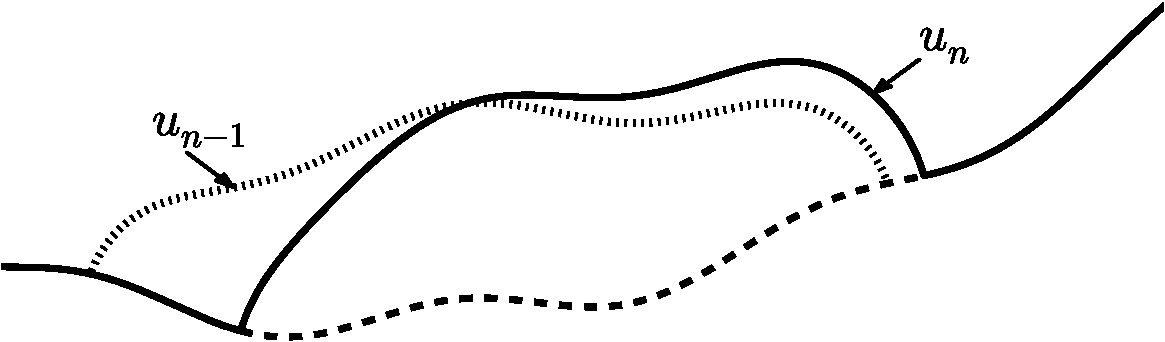
\includegraphics[width=3.9in,keepaspectratio=true]{time-step-cartoon}
\end{center}
\caption{The single time-step problem of \eqref{eq:semimassconserve} and \eqref{eq:semiconstraint} is a free boundary problem determining a new thickness $u_n\ge 0$ from an old thickness $u_{n-1}$ and from the source term $F_n$ during the time step.}
\label{fig:timestepcartoon}
\end{figure}

The semi-discretization procedure which generates equations \eqref{eq:semimassconserve} and \eqref{eq:semiconstraint} produces functions
\begin{equation}
\bQ_n(\bX,v,x), \quad F_n(v,x) \label{eq:functionalforms}
\end{equation}
Here $\bX\in\RR^d$ is any vector, $v\in\RR$, and $x\in \Omega$.  We will assume $\bQ_n$ is defined for all $x\in\Omega$, not just where $v(x)>0$, but that $\bQ_n(\bX,0,x)=0$ because a zero-thickness layer moves no mass (subsection \ref{subsec:fluxassumptions}).

\subsection{$\theta$ methods}  \label{subsec:thetamethods}  In the simplest implicit case, namely using a backward Euler scheme applied to \eqref{eq:massconserve} and \eqref{eq:constraint}, we have $\bQ_n = \bq(\bX,v,x,t_n)$ and $F_n = f(v,x,t_n)$.  However, according to the particular discretization procedure, the source function $F_n$ ``absorbs'' all the terms which do not involve the flux $\bq$ evaluated at time $t_n$.

For example, consider a $\theta$-method discretization \cite{MortonMayers2005} of \eqref{eq:massconserve} with $0\le \theta \le 1$:
\begin{align}
  &\frac{u_n - u_{n-1}}{\Delta t_n} + \theta\, \Div \bq(\grad u_n,u_n,x,t_n) + (1-\theta) \Div \bq(\grad u_{n-1},u_{n-1},x,t_{n-1}) \label{eq:thetamethod} \\
  &\qquad =  \theta f(u_n,x,t_n) + (1-\theta) f(u_{n-1},x,t_{n-1}). \notag
\end{align}
The $\theta=0$ case of \eqref{eq:thetamethod} is the forward Euler method, $\theta=1/2$ is trapezoid (Crank-Nicolson), and $\theta=1$ is backward Euler.  Equation \eqref{eq:thetamethod} is of form \eqref{eq:semimassconserve} with
\begin{align*}
\bQ_n(\bX,v,x) &= \theta\, \bq(\bX,v,x,t_n), \\
F_n(v,x)       &= \theta f(v,x,t_n) + (1-\theta) f(u_{n-1},x,t_{n-1}) \\
               &\qquad - (1-\theta) \Div \bq(\grad u_{n-1},u_{n-1},x,t_{n-1}).
\end{align*}
If $\theta=0$ then $\bQ_n=0$; yes, this case is allowed in our weakly-posed theory (section \ref{sec:weakform}).  However, implicitness is both helpful for the usual stability reasons \cite{MortonMayers2005} and additionally so as to give the smoothness needed so that the weak form of the single time-step problem can be well-posed; see section \ref{sec:weakform} and subsection \ref{subsec:explicit}.

Time-discretization need not be limited to $\theta$-methods.  In particular, multi-stage one-step schemes like Runge-Kutta can be put in the form of \eqref{eq:semimassconserve}---see Appendix \ref{app:rk2}.  Multi-step integration methods also fit into our framework (not shown), but the low regularity of the solution in the vicinity of the free boundary suggests thus such schemes may provide no accuracy improvement.

\subsection{Associated set decomposition}  \label{subsec:setdecompose}  Suppose that the above single time-step problem is well-posed.  We can then decompose $\Omega$ using the solution of problem \eqref{eq:semimassconserve} and \eqref{eq:semiconstraint}, defining three disjoint regions based on $u_n$ and $u_{n-1}$:
\begin{align*}
\Omega_n &= \left\{x \in \Omega \,\big|\, u_n(x)>0\right\}, \\
\Omega_n^r &= \left\{x \in \Omega \,\big|\, u_n(x)=0 \text{ and } u_{n-1}(x) > 0\right\}, \\
\Omega_n^0 &= \left\{x \in \Omega \,\big|\, u_n(x)=0 \text{ and } u_{n-1}(x) = 0\right\},
\end{align*}
so that
\begin{equation}
\Omega = \Omega_n \cup \Omega_n^r \cup \Omega_n^0.  \label{eq:omegadecomposition}
\end{equation}
Here the superscript ``$r$'' stands for ``retreat,'' and $\Omega_n^r$ is called the \emph{retreat set}.  Figure \ref{fig:domains} illustrates this decomposition in the planar case ($\Omega \subset \RR^2$).  If $u_n$ is continuous then $\Omega_n$ is open, in which case sets $\Omega_n^r \cup \Omega_n^0$ and $\Omega_n^0$ are closed in $\Omega$.

\begin{figure}[ht]
\medskip
\begin{center}
\includegraphics[width=2.3in,keepaspectratio=true]{domains-fig}
\end{center}
\caption{We decompose $\Omega = \Omega_n \cup \Omega_n^r \cup \Omega_n^0$, where $\Omega_n$ is the support of $u_n$, $\Omega_n^r$ is the retreat set, and $\Omega_n^0$ is the set on which both $u_{n-1}$ and $u_n$ are zero.}
\label{fig:domains}
\end{figure}

Assume $F_n(v,x)$ and $u_n(x)$ are continuous.  Rewriting \eqref{eq:semimassconserve} as
\begin{equation}
u_n = u_{n-1} + \Delta t_n\, F_n - \Delta t_n\, \Div \bQ_n,  \label{eq:strongflat}
\end{equation}
we see that if $u_n=0$ then the terms on the right side of \eqref{eq:strongflat} must, apparently, either sum to zero or be negative, as otherwise they would be balanced by a positive value for $u_n$.  Furthermore, we will assume (see \eqref{eq:Qiszero} below) that the flux of a zero-thickness layer is zero, so $\bQ_n=0$ on $\Omega_n^r \cup \Omega_n^0$ where $u_n=0$.  Because also $u_{n-1}\ge 0$ and $\Delta t_n > 0$, we expect that on $\Omega_n^r \cup \Omega_n^0$ this inequality holds:
\begin{equation}
u_{n-1} + \Delta t_n\, F_n \le 0. \label{eq:strongconditionwherezero}
\end{equation}
Note \eqref{eq:strongconditionwherezero} implies $F_n \le 0$ on $\Omega_n^r \cup \Omega_n^0$ as well.

The intuition behind \eqref{eq:strongconditionwherezero}, which will be used in deriving the weak form, is that the source term must be sufficiently negative in a thickness-zero location where the layer was previously present (i.e.~in $\Omega_n^r$), or where it continues to be absent (in $\Omega_n^0$).


\section{Weak formulation of the single time-step problem}  \label{sec:weakform}  The strong form \eqref{eq:semimassconserve} and \eqref{eq:semiconstraint} of the single time-step problem is not, however, adequate for further mathematical progress.  PDE \eqref{eq:semimassconserve} applies on the set where its solution $u_n$ is positive (i.e.~on $\Omega_n$).  Likewise, inequality \eqref{eq:strongconditionwherezero} specifies behavior on the set where $u_n=0$.  We have in fact ``posed'' a problem in terms of its solution.  The strong form is also inadequate because the boundary conditions satisfied by the solution $u_n$ along the free boundary $\partial\Omega_n$ are not clear.

By contrast, a weak form of the single time-step problem can be well-posed.  Our weak form in this section is a variational inequality \cite{Friedman1982,KinderlehrerStampacchia1980} on a convex set of admissible functions.  This formulation refers only to the set $\Omega$ and its boundary $\partial\Omega$, not to $\Omega_n$.

We will state conditions on the discrete-time flux $\bQ_n$ first (subsection \ref{subsec:fluxassumptions}), then construct a variational inequality (subsection \ref{subsec:derivevi}), and then show that a sufficiently-smooth solution of this weak problem solves the strong problem (subsection \ref{subsec:interior}).  Section \ref{sec:wellposed} addresses well-posedness, which depends on details of $\bQ_n$ that are not included in the current section.

\subsection{Flux and source assumptions} \label{subsec:fluxassumptions}  Let $p\ge 1$ and recall that $L^p (\Omega)$ is the Banach space of functions with norm $\|v\|_{L^p} = \left(\int_\Omega |v|^p\,dx\right)^{1/p}$.  The Sobolev space $W^{1,p}(\Omega)$ is the Banach space of functions $v$ with $v,\partial_1 v,\dots,\partial_d v \in L^p(\Omega)$ \cite{Evans1998}, with norm
\begin{equation}
  \|v\|_{1,p} = \left(\|v\|_{L^p}^p + \sum_i \|v\|_{L^p}^p\right)^{1/p}.  \label{eq:norm}
\end{equation}
If $p>d$ then each $v\in W^{1,p}(\Omega)$ has a continuous representative \cite[``Morrey's inequality'']{Evans1998}, but otherwise $v$ may be discontinuous.  Denote by $W_0^{1,p}(\Omega)$ the closure of $C_c^\infty(\Omega)$ in $W^{1,p}(\Omega)$.  For $v \in W^{1,p}(\Omega)$ define $E_v = \{x\in\Omega \,\big|\, v(x) = 0\}$.  Note that $\grad v = 0$ a.e.~on $E_v$ \cite[lemma A.4 in chapter II]{KinderlehrerStampacchia1980}.  Also let $q=(1-1/p)^{-1}$.

\medskip
\begin{definition}  \label{ass:std}  We say $\bQ_n$ satisfies the \emph{standard flux assumptions} if
\renewcommand{\labelenumi}{\emph{\roman{enumi}})}
\begin{enumerate}
\item for each fixed $x\in \Omega$,
\begin{equation}
(\bX,z) \mapsto \bQ_n(\bX,z,x) \text{ is continuous on } \RR^d \times \RR,  \label{eq:Qiscontinuous}
\end{equation}
\item if $v \in W^{1,p}(\Omega)$ then
\begin{equation}
\bQ_n(\grad v,v,x) \in L^q(\Omega), \label{eq:QisLq}
\end{equation}
\item
\begin{equation}
\bQ_n(\grad v,v,x)=0 \quad \text{a.e.~on } E_v. \label{eq:Qiszero}
\end{equation}
\end{enumerate}
\end{definition}

In summary, assumptions \eqref{eq:Qiscontinuous} and \eqref{eq:QisLq} require $\bQ_n$ to be a well-behaved function, while \eqref{eq:Qiszero} says that $\bQ_n=0$ if the thickness is zero, as it is the flux of a layer.  Regarding the source term $F_n$, in all of section \ref{sec:weakform} we assume only that if $v\in W^{1,p}(\Omega)$ then
\begin{equation}
F_n(v,x) \in L^q(\Omega).  \label{eq:FisLq}
\end{equation}


\subsection{Derivation of the variational inequality}  \label{subsec:derivevi}  To use the strong form in deriving a weak form (and vice versa; see subsection \ref{subsec:interior}), we need an extra assumption that $\bQ_n$ is smooth:  For all open $S \subset \Omega$, if $v\in W^{1,p}(S)$ then
\begin{equation}
\frac{\partial}{\partial x_i} \bQ_n(\grad v,v,x) \in L^q(S). \label{eq:Qissmooth}
\end{equation}
This assumption will not affect our later considerations of well-posedness (section \ref{sec:wellposed} or conservation errors (sections \ref{sec:timeseries}) and \ref{sec:spacediscretized}).

\medskip
\begin{theorem} \label{thm:strongimpliesweak}  Suppose $u_n\ge 0$ solves \eqref{eq:semimassconserve} on $\Omega_n$ and \eqref{eq:strongconditionwherezero} on $\Omega_n^r \cup \Omega_n^0$.  Suppose $u_n,v\in C(\overline{\Omega})$, $v\ge 0$, and $\grad u_n,\grad v \in L^p(\Omega)$.  Suppose the boundaries of the sets $\Omega_n$ and $\Omega_n^r \cup \Omega_n^0$ in decomposition \eqref{eq:omegadecomposition} are all sufficiently smooth (e.g.~Lipshitz).  Suppose $\bQ_n$ satisfies the standard flux assumptions and \eqref{eq:Qissmooth}.  Suppose $F_n$ satisfies \eqref{eq:FisLq}.  Write $\bQ_n=\bQ_n(\grad u_n,u_n,x)$ and $F_n = F_n(u_n,x)$.  Then
\begin{equation}
-\int_{\Omega} \bQ_n \cdot \grad(v-u_n) \ge \int_{\Omega} \left(F_n - \frac{u_n - u_{n-1}}{\Delta t}\right) (v-u_n). \label{eq:morallytheVI}
\end{equation}
\end{theorem}

\begin{proof}  Let $w=v-u_n$.  Using decomposition \eqref{eq:omegadecomposition} and integration by parts---here we use regularity of $\partial \Omega_n$ and $\partial(\Omega_n^r \cup \Omega_n^0)$ and assumption \eqref{eq:Qissmooth} on $S=\Omega_n$ and $S=(\Omega_n^r \cup \Omega_n^0)^\circ$---we get
\begin{align}
-\int_{\Omega} \bQ_n \cdot \grad w &= \int_{\Omega_n} (\Div \bQ_n) w - \int_{\partial \Omega_n} (\bQ_n \cdot \bn) w \label{eq:intbypartsfromstrong} \\
  &\qquad\quad + \int_{\Omega_n^r \cup \Omega_n^0} (\Div \bQ_n) w - \int_{\partial(\Omega_n^r \cup \Omega_n^0)} (\bQ_n \cdot \bn) w. \notag
\end{align}
Because $u_n$ is continuous, $u_n=0$ on $\partial \Omega_n$ and on $\partial(\Omega_n^r \cup \Omega_n^0)$.  Thus by \eqref{eq:Qiscontinuous} and \eqref{eq:Qiszero} we see that $\bQ_n=0$ on these boundaries, so the boundary integrals in \eqref{eq:intbypartsfromstrong} are zero.  Now, by \eqref{eq:semimassconserve} on $\Omega_n$, and by \eqref{eq:Qiszero} and \eqref{eq:Qissmooth} we have $\Div \bQ_n=0$ on $\Omega_n^r \cup \Omega_n^0$.  Thus we get
\begin{equation}
-\int_{\Omega} \bQ_n \cdot \grad w = \int_{\Omega_n} \left(F_n - \frac{u_n - u_{n-1}}{\Delta t}\right) w. \label{eq:equalitybeforeVI}
\end{equation}
However, by \eqref{eq:strongconditionwherezero}, $F_n \le 0$ on $\Omega_n^r \cup \Omega_n^0$.  Since also $u_n=0$, $u_{n-1}\ge 0$, and $w = v-u_n = v \ge 0$ on $\Omega_n^r \cup \Omega_n^0$, we have
\begin{equation}
    0 \ge \int_{\Omega_n^r \cup \Omega_n^0} \left(F_n - \frac{u_n - u_{n-1}}{\Delta t}\right) w. \label{eq:inequalitybeforeVI}
\end{equation}
Adding \eqref{eq:equalitybeforeVI} and \eqref{eq:inequalitybeforeVI} gives \eqref{eq:morallytheVI}.
\end{proof}

While this derivation of inequality \eqref{eq:morallytheVI} requires too many hypotheses, it serves as adequate motivation to define our weak problem.  Inequality \eqref{eq:morallytheVI} can serve as the weak problem because it avoids using the solution to define subsets of $\Omega$ on which pointwise equalities or inequalities apply.  Statement \eqref{eq:morallytheVI} also requires less regularity of $u_{n-1}$ and $u_n$ than needed for strong form \eqref{eq:semimassconserve}.

For the next definition, fix $p>1$ and denote $\mathcal{X} = W_0^{1,p}(\Omega)$ with norm $\|\cdot\|$.  Denote its dual space by $\mathcal{X}'$ and $\ip{\cdot}{\cdot}: \mathcal{X}' \times \mathcal{X} \to \RR$ for the pairing.

\begin{definition}  \label{def:spaces}
    $$\mathcal{K} = \left\{v \in \mathcal{X} \,\big|\, v(x) \ge 0 \text{ a.~e.~} x \in \Omega\right\},$$
a closed and convex subset of $\mathcal{X}$.
\end{definition}

\begin{definition}  Suppose $u_{n-1}\in\mathcal{K}$ and $\Delta t_n>0$.  Assume that $\bQ_n$ satisfies the standard flux assumptions and that $F_n$ satisfies \eqref{eq:FisLq}.  Define $A_n:\mathcal{K} \to \mathcal{X}'$ by
\begin{equation}
  \ip{A_n(v)}{\phi} = \int_\Omega \left(v - \Delta t\, F_n(v,x) - u_{n-1}\right)\phi - \Delta t_n\, \bQ_n(\grad v,v,x) \cdot \grad\phi. \label{eq:defineAn}
\end{equation}
\end{definition}

\begin{definition}  We say $u_n$ solves the \emph{(weak form) single time-step problem} if
\begin{equation}
  \ip{A_n(u_n)}{v-u_n} \ge 0 \quad \text{for all } v \in \mathcal{K}.  \label{eq:theVI}
\end{equation}
\end{definition}

Of course, \eqref{eq:theVI} is the same inequality as \eqref{eq:morallytheVI}.


\subsection{Interior condition}  \label{subsec:interior}  We can further justify the weak form by showing a converse of Theorem \ref{thm:strongimpliesweak}.  Note that we make no regularity assumptions related to the sets \eqref{eq:omegadecomposition}.

\medskip
\begin{theorem} \label{thm:weakimpliesstrong}  Assume $\bQ_n$ satisfies the standard flux assumptions and \eqref{eq:Qissmooth}, and assume $F_n$ satisfies \eqref{eq:FisLq}.  Suppose $u_n\in\mathcal{K}$ solves the single-time-step weak problem \eqref{eq:theVI}.
\renewcommand{\labelenumi}{\emph{(\roman{enumi})}}
\begin{enumerate}
\item If $S \subset \Omega_n$ is open, $\overline{S}\subset \Omega$, $u_n\in C(S)$, and $u_n(x)>0$ for all $x\in S$, then equation \eqref{eq:semimassconserve} applies a.e.~$x\in S$.
\item If $S \subset \Omega_n^0$ is open then $u_{n-1} + \Delta t_n\,F_n \le 0$, and thus $F_n \le 0$, a.e.~$x\in S$.
\end{enumerate}
\end{theorem}

\medskip
\begin{proof}  To prove (i) choose any $\phi\in C_c^\infty(S)$ and extend it by zero to all of $\Omega$; note that $\phi$ can have either sign, but that $\phi=0$ on $\partial\Omega$.  Let $v = u_n + \eps \phi$ and note that $v \in \mathcal{K}$ as long as $\eps\in\RR$ is sufficiently small in magnitude.  Specifically, $v \in \mathcal{K}$ if $|\eps|\le \eps_0$ where $\eps_0 = \min u_n(x) / \max |\phi(x)| > 0$, with the minimum and maximum taken over the (compact) closure of the support of $\phi$.  It follows from \eqref{eq:theVI} that
   $$\eps \int_\Omega \left(u_n - \Delta t_n\,F_n - u_{n-1}\right)\phi - \Delta t_n\,\bQ_n \cdot \grad \phi \ge 0.$$
This is true for all $-\eps_0 \le \eps \le \eps_0$, so the integral is zero.  Integration by parts, using assumption \eqref{eq:Qissmooth} and $\phi\big|_{\partial\Omega}=0$, gives
   $$\int_\Omega \left[ u_n - \Delta t_n\,F_n - u_{n-1} + \Delta t_n\,\Div\bQ_n \right]\phi = 0.$$
Because $\phi\in C_c^\infty(S)$ is arbitrary, the quantity in square brackets is zero a.e.~as claimed.

To prove (ii) we start with nonnegative $\phi\in C_c^\infty(S)$, extend it by $\phi$ by zero, and let $v = u_n + \phi$ so $v\in\mathcal{K}$.  Because $S\subset \Omega_n^r\cup\Omega_n^0$, $u_n=0$ on the support of $\phi$.  By assumptions \eqref{eq:Qiscontinuous} and \eqref{eq:Qiszero}, $\bQ_n=0$ on the support of $\phi$ also.  Thus by \eqref{eq:theVI},
    $$0 \ge \int_{\Omega} \left(u_{n-1} + \Delta t_n\, F_n\right) \phi,$$
and it follows as before that $u_{n-1} + \Delta t_n\, F_n \le 0$ a.e.~on $S$.\end{proof}

\medskip
Thus a continuous weak solution $u_n$ of \eqref{eq:theVI} solves PDE \eqref{eq:semimassconserve} where it is positive, and otherwise it satisfies inequalities \eqref{eq:strongconditionwherezero}.  From now on we will use set decomposition \eqref{eq:omegadecomposition} when referring to a solution $u_n$ of the weak form \eqref{eq:theVI}.


\section{\emph{A posteriori} analysis of mass conservation on the free boundary}  \label{sec:timeseries}

From now on until section \ref{sec:wellposed} we assume that the weak problem for a single time-step, i.e.~\eqref{eq:theVI}, is well-posed.  In particular, given an initial state $u_0\in\mathcal{K}$ there is a unique sequence $\{u_n\}_1^N \subset \mathcal{K}$ which solves the $n=1,\dots,N$ problems \eqref{eq:theVI}.

Define
\begin{equation}
M_n = \int_\Omega u_n(x)\,dx = \int_{\Omega_n} u_n(x)\,dx \ge 0, \label{eq:totalmassseries}
\end{equation}
the \emph{(total) mass} at time $t_n$, and define
\begin{equation}
C_n = \Delta t_n\, \int_{\Omega_n} F_n(u_n,x)\,dx, \label{eq:climateseries}
\end{equation}
the \emph{climate input} during the $n$th time step.  Note that the climate input $C_n$ into the fluid layer is computed by integration over locations where the fluid exists ($\Omega_n$), and not over all of $\Omega$, nor over where the fluid previously existed ($\Omega_{n-1}$).

Practical models compute approximations to time-series $M_n$ and $C_n$ as model outputs, so as to help a model user model mass transfers.  A well-implemented numerical model of a fixed-boundary fluid layer problem would achieve exact discrete mass conservation in the sense that
\begin{equation}
M_n = M_{n-1} + C_n \label{eq:oldbalance}
\end{equation}
at each time $t_n$, to within rounding error.  That is, one can easily show \eqref{eq:oldbalance} under a Neumann condition $\bQ_n=0$ on $\partial \Omega$ in strong problem \eqref{eq:semimassconserve} if $\Omega_n=\Omega$.  Under additional fluid-layer-type assumptions \eqref{eq:Qiscontinuous} and \eqref{eq:Qiszero}, which force the flux to zero at the boundary because the thickness $u_n$ goes to zero there, \eqref{eq:oldbalance} also holds under a Dirichlet condition $u_n\in W_0^{1,p}(\Omega)$ if $\Omega_n=\Omega$.  However, balance \eqref{eq:oldbalance} does not follow from definitions \eqref{eq:totalmassseries} and \eqref{eq:climateseries} when there is a free boundary, that is, when $\Omega_n \subsetneq \Omega$.

To quantify the situation for the free-boundary case, recall $\Omega_n^r$ is the retreat set in the $n$th time-step (subsection \ref{subsec:setdecompose}).  Define
\begin{equation}
R_n = \int_{\Omega_n^r} u_{n-1}\,dx \ge 0, \label{eq:retreatlossseries}
\end{equation}
which we call the \emph{retreat loss} during the $n$th time step.  Then by \eqref{eq:semimassconserve} we have
\begin{align}
M_n - M_{n-1} &= \int_{\Omega_n} (u_n - u_{n-1})\,dx + \int_{\Omega_n^r} (0 - u_{n-1})\,dx \label{eq:newbalance} \\
   &= \Delta t \int_{\Omega_n} (- \Div \bQ_n + F_n) \,dx \, - R_n \notag \\
   &= C_n - R_n \notag
\end{align}
because $\bQ_n=0$ along $\partial \Omega_n$ by \eqref{eq:Qiscontinuous} and \eqref{eq:Qiszero}.

The distinction between \eqref{eq:oldbalance} and \eqref{eq:newbalance} is a major point of our paper.  That is, the achievable space-integrated mass conservation statement for free-boundary problems at each time-step is the new \emph{a posteriori} statement \eqref{eq:newbalance}.  Computing $R_n$, or an equivalent quantity, is thus an essential step in understanding moving-boundary models of fluid motion.  Furthermore, the retreat loss $R_n$ can be bounded \emph{a priori} if we have additional information about the solution of variational inequality \eqref{eq:theVI}.  This would allow approximation of the earlier, preferred mass conservation relation \eqref{eq:oldbalance} to within some tolerance.

In particular, consider the solution of \eqref{eq:theVI} for time step $\Delta t>0$.  By Theorem \ref{thm:weakimpliesstrong} (ii) we have
\begin{equation}
R_n \le - \Delta t\,\int_{\Omega_n^r} F_n(u_n,x)\,dx  \label{eq:earlyretreatbound}
\end{equation}
because $u_{n-1} + \Delta t\,F_n \le 0$ a.e.~in $\Omega_n^r$.

FIXME Assume that $F_n$ is uniformly Lipshitz as a function of $v$: there is $L>0$ so that for all $x\in\Omega$ and $v_1,v_2 \in [0,\infty)$, we have
\begin{equation}
\left|F_n(v_1,x)-F_n(v_2,x)\right| \le L |v_1-v_2|.  \label{eq:Fislip}
\end{equation}
In particular, $F_n$ is continuous as a function of $v$.

If we also assume Lipshitz continuity \eqref{eq:Fislip} for $F_n$, and we assume there is a stability bound
\begin{equation}
\|u_n-u_{n-1}\|_{L^1(\Omega)} \le \Phi_n(\Delta t)
\end{equation}
for some bounded function $\Phi_n : [0,\infty) \to [0,\infty)$, then
\begin{equation}
R_n \le \Delta t\,\left(C_{n-1} + L \Phi_n(\Delta t)\right),   \label{eq:retreatbound}
\end{equation}
for a constant $C_{n-1}=\left|\int_{\Omega} F_n(u_{n-1},x)\,dx\right|$ which is computable \emph{a priori} on each single time-step problem \eqref{eq:theVI}.  If $\Phi_n$ is bounded by $M>0$, or better if $\Phi_n(z) \le A \Delta t^q$ for $A,q>0$, then a time-step $\Delta t=\Delta t_n$ can be computed so that $R_n$ is less than a desired tolerance.

As an operational statement about discrete-time models, we can rephrase our major assertion from the Introduction as
\begin{quote}
\emph{The model for a moving-boundary fluid layer should store a time series for $R_n$, in addition to the expected time series $C_n$, in order to provide auditable mass conservation.}
\end{quote}
In stating this assertion, we note that the retreat loss $R_n$ should vanish in the $\Delta t_n\to 0$ limit, which is a consistency statement about the time-discretized model, and that we can show $R_n\to 0$ in that limit with additional stability results on the solution of the weak single time-step problem \eqref{eq:theVI}.


\section{The fully-discrete single time-step problem}  \label{sec:spacediscretized}

So far we have treated time-dependent free-boundary mass conservation models in time-semi-discretized form, as a sequence of continuous-space free-boundary problems.  We will address well-posedness (section \ref{sec:wellposed}) in such a continuous-space framework also.  However, considering the fully-discrete case shows that we must add to the \emph{a posteriori} computations of the last section if we are to completely balance the conservation books at the free boundary.

In this section we make the mild assumption that the spatial discretization allows an unstructured finite volume \cite{LeVeque2002} interpretation (subsection \ref{subsec:spacenotation}), and this is sufficient to give a fully-discrete balance analogous to the continuous-space version \eqref{eq:newbalance} above (subsection \ref{subsec:shellerror}).  After that we consider numerical solution methods for the constrained nonlinear problem (subsection \ref{subsec:newtonvi}).

\subsection{Unstructured finite volume method} \label{subsec:spacenotation}  First we set notation for a generic finite volume scheme.  We restrict to $\Omega \subset \RR^d$, for $d=2,3$, which is an open polygon (polyhedron).  We assume that $\Omega$ is tiled by finitely-many open polygonal (polyhedral) cells $\omega_j$, indexed by $j\in J$, with area (volume) $|\omega_j|=a_j$.  These cells may be non-convex and the number of edges (faces) per cell may vary.  Because this is a tiling, $\omega_j \cap \omega_k = \emptyset$ for $j\ne k$ and
\begin{equation}
\bar\Omega = \bigcup_{j\in J} \bar \omega_j \quad \text{and} \quad |\Omega| = \sum_{j\in J} a_j.  \label{eq:tiling}
\end{equation}
An edge (face), simply denoted by the ordered pair $(j,k)$, exists between cell $j$ and cell $k$ if $\bar\omega_j \cap \bar \omega_k$ has positive $d-1$ measure (i.e.~length or area) $\ell_{(j,k)}>0$.  The set of edges $(j,k)$ for cell $\omega_j$ is denoted $\mathcal{E}_j$.

Our approach is now to discretize the strong form equation \eqref{eq:semimassconserve} using finite volume ideas, but this can be treated as a non-conforming Petrov-Galerkin finite element method for the variational inequality \eqref{eq:theVI} with $A_n$ defined by \eqref{eq:defineAn}.  In that case the test functions are piecewise-constant and discontinuous along the edges of the cells $\omega_j$, as in a so-called ``finite volume element'' method \cite{Bueler2016,Cai1990,EwingLinLin2002}.  The cells $\omega_j$ might be geometrically ``dual'' to the elements in such a scheme (e.g.~\cite{Ringleretal2013}).

The representative thickness $u_n^j$ in cell $j$ is given the usual finite volume definition as an average \cite{LeVeque2002}, and similarly $F_n^j$ denotes a representative source term for the cell:
\begin{equation}
u_n^j \approx \frac{1}{a_j} \int_{\omega_j} u_n(x), \qquad F_n^j \approx \frac{1}{a_j} \int_{\omega_j} F_n(u_n,x).  \label{eq:fvthickness}
\end{equation}
The value $F_n^j$ is computed by some quadrature scheme as necessary, but the details do not matter here.  The discrete (scalar) normal flux across the edge $(j,k)$, outward from cell $j$, is denoted
\begin{equation}
Q_n^{(j,k)} \approx \frac{1}{\ell_{(j,k)}} \int_{(j,k)} \bQ_n \cdot \bn_{(j,k)}, \label{eq:fvflux}
\end{equation}
as shown Figure \ref{fig:fvmesh-notation}, where $\bn_{(j,k)}$ denotes the unit normal vector to edge $(j,k)$ directed outward from $\omega_j$.  We assume that these fluxes are approximated by some scheme, based on values $\{u_n^l\}$ for $l$ potentially ranging over the entire mesh.  Though the details are not important here, these discrete fluxes might be computed by upwinded and/or flux-limited schemes \cite{LeVeque2002} according to the functional form of the flux $\bQ_n$.

\begin{figure}[ht]
\begin{center}
% created by hand
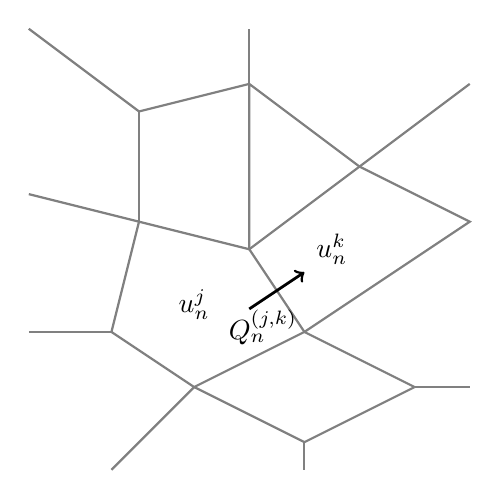
\begin{tikzpicture}[scale=0.35]
  %uncomment to see grid on which it was generated:
  %\draw[dotted,step=1.0,black,very thin] (0,0) grid (16,16);

    % exterior cell boundaries
  \draw[gray, thick] (3,0) -- (6,3);
  \draw[gray, thick] (0,5) -- (3,5);
  \draw[gray, thick] (0,10) -- (4,9);
  \draw[gray, thick] (0,16) -- (4,13);
  \draw[gray, thick] (4,13) -- (4,9);
  \draw[gray, thick] (4,13) -- (8,14);
  \draw[gray, thick] (8,14) -- (8,16);
  \draw[gray, thick] (12,11) -- (16,14);
  \draw[gray, thick] (10,5) -- (14,3);
  \draw[gray, thick] (10,1) -- (14,3);
  \draw[gray, thick] (14,3) -- (16,3);
  \draw[gray, thick] (6,3) -- (10,1);
  \draw[gray, thick] (10,0) -- (10,1);
  % interior cell boundaries
  \draw[gray, thick] (10,5) -- (8,8);
  \draw[gray, thick] (8,8) -- (12,11);



  % the free boundary is just like the other edges
  \draw[gray, thick] (6,3) -- (3,5) -- (4,9) -- (8,8) -- (8,14) --
              (12,11) -- (16,9) -- (10,5) -- cycle;
  % label some cell d.o.f.
  \draw (6,6) node {$u_n^j$};
  \draw (11,8) node {$u_n^k$};
  % show normal flux
  \def\xmid{9};
  \def\ymid{6.5};
  \def\dx{3/3};
  \def\dy{2/3};
  \draw[->,line width=1.0pt] (\xmid-\dx,\ymid-\dy) -- (\xmid+\dx,\ymid+\dy); % normal vector
  \draw (\xmid-\dx/2,\ymid-2*\dy) node {$Q_n^{(j,k)}$}; % label as flux
\end{tikzpicture}

\end{center}
\caption{Notation for an unstructured finite volume method for \eqref{eq:semimassconserve} in $\RR^2$.}
\label{fig:fvmesh-notation}
\end{figure}

We make only two specific assumptions about the fully-discrete finite volume scheme:
\renewcommand{\labelenumi}{(\roman{enumi})}
\begin{enumerate}
\item There is local conservation between any two adjacent cells which are fluid-filled:
\begin{equation}
  u_n^j u_n^k > 0 \quad \implies \quad Q_n^{(k,j)}=-Q_n^{(j,k)}.  \label{eq:fvlocalconservation}
\end{equation}
\item If $u_n^j>0$ then the strong form single-time-step problem \eqref{eq:semimassconserve} is approximated by
\begin{equation}
\frac{u_n^j - u_{n-1}^j}{\Delta t_n} + \frac{1}{a_j} \sum_{k\in \mathcal{E}_j} Q_n^{(j,k)} \ell_{(j,k)} = F_n^j. \label{eq:fvmassconserve}
\end{equation}
\end{enumerate}

Local discrete conservation statement (i) is completely standard, but the fluid-filled hypothesis is important.  We do not expect discrete conservation in the sense $Q_n^{(k,j)}=-Q_n^{(j,k)}$ at the free boundary because a flux scheme at the edge (face) of a fluid-free cell, facing a fluid-filled cell, cannot be expected to generate flux which is compatible with monotonicity or coercivity properties (subsection \ref{subsec:mono} below) which would lead to well-posedness.

Regarding (ii), recall that, at least heuristically, the divergence of a vector field $\bX$ is the limit of line (surface) integrals, $|R|^{-1} \int_{\partial R} \bX\cdot \bn \to \Div \bX$, where $R\subset \RR^d$ denotes a sequence of regions with Lipshitz boundary, enclosing and shrinking down to $x$, with outward unit normal vector $\bn$.  Though \eqref{eq:fvmassconserve} requires the discrete scheme to approximate such an integral, this prescription has great flexibility because of the many possible meanings of approximations \eqref{eq:fvthickness}--\eqref{eq:fvflux}.

Many schemes can be given interpretations \eqref{eq:fvthickness}--\eqref{eq:fvmassconserve}, including structured-grid (i.e.~uniform rectangular cell) finite difference \cite{Bueler2016,MortonMayers2005} and structured/unstructured finite volume \cite{LeVeque2002} schemes.  A framework for unstructured-grid finite volume schemes, compatible with the fixed-boundary version of the above setup, has been implemented for ocean modeling \cite{Ringleretal2013}.

\subsection{The discrete-space ``shell error''}  \label{subsec:shellerror}  In the fully-discrete model we use a superscript ``$h$'' to denote the spatially-discrete version of integrated quantities.  That is, analogous to \eqref{eq:totalmassseries}, \eqref{eq:climateseries}, and \eqref{eq:retreatlossseries}, we define the time-series
\begin{equation}
  M_n^h = \sum_j u_n^j a_j, \quad C_n^h = \Delta t_n\!\!\sum_{\{j:u_n^j>0\}} F_n^j a_j, \quad \text{ and } \quad R_n^h = \sum_{\{j:u_n^j=0\}} u_{n-1}^j a_j.  \label{eq:fvtimeseriesdefn}
\end{equation}
Analogous to \eqref{eq:newbalance}, by \eqref{eq:fvmassconserve} we compute
\begin{align}
M_n^h - M_{n-1}^h &= \sum_{u_n^j>0} (u_n^j - u_{n-1}^j) a_j - \sum_{u_n^j=0} u_{n-1}^j a_j \notag \\
   &= - \Delta t_n\,\sum_{u_n^j>0}\, \sum_{(j,k)\in\mathcal{E}_j} Q_n^{(j,k)} \ell_{(j,k)} + \Delta t_n\,\sum_{u_n^j>0} F_n^j a_j - R_n^h \notag \\
   &= - \Delta t_n\,\sum_{u_n^j>0}\, \sum_{(j,k)\in\mathcal{E}_j} Q_n^{(j,k)} \ell_{(j,k)} + C_n^h - R_n^h.  \label{eq:fvnewbalance}
\end{align}

Though in the continuous-space version \eqref{eq:newbalance} we could eliminate the flux integral, the remaining discrete flux sum in \eqref{eq:fvnewbalance} is not zero.  Local conservation \eqref{eq:fvlocalconservation} only reduces it to a sum over edges which have a positive-thickness cell on one side and a zero-thickness cell on the other.  We call this free-boundary discrete-flux residual sum the \emph{shell error}:
\begin{equation}
S_n^h = \sum_{u_n^j>0}\, \sum_{(j,k)\in\mathcal{E}_j} Q_n^{(j,k)} \ell_{(j,k)} = \sum_{u_j^n > 0 \,\&\, (j,k)\in\mathcal{E}_j \,\&\, u_k^n = 0} Q_n^{(j,k)} \ell_{(j,k)} \label{eq:fvderiveshellerror}
\end{equation}

\begin{figure}[ht]
\begin{center}
% created by hand
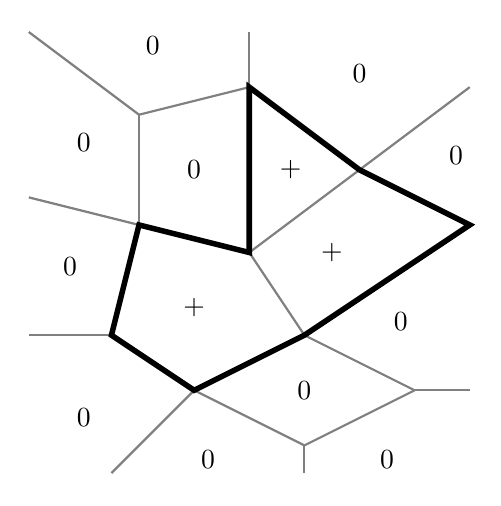
\begin{tikzpicture}[scale=0.35]
  %uncomment to see grid on which it was generated:
  %\draw[dotted,step=1.0,black,very thin] (0,0) grid (16,16);

    % exterior cell boundaries
  \draw[gray, thick] (3,0) -- (6,3);
  \draw[gray, thick] (0,5) -- (3,5);
  \draw[gray, thick] (0,10) -- (4,9);
  \draw[gray, thick] (0,16) -- (4,13);
  \draw[gray, thick] (4,13) -- (4,9);
  \draw[gray, thick] (4,13) -- (8,14);
  \draw[gray, thick] (8,14) -- (8,16);
  \draw[gray, thick] (12,11) -- (16,14);
  \draw[gray, thick] (10,5) -- (14,3);
  \draw[gray, thick] (10,1) -- (14,3);
  \draw[gray, thick] (14,3) -- (16,3);
  \draw[gray, thick] (6,3) -- (10,1);
  \draw[gray, thick] (10,0) -- (10,1);
  % interior cell boundaries
  \draw[gray, thick] (10,5) -- (8,8);
  \draw[gray, thick] (8,8) -- (12,11);



  % the free boundary is bold
  \draw[line width=2.0pt] (6,3) -- (3,5) -- (4,9) -- (8,8) -- (8,14) --
                          (12,11) -- (16,9) -- (10,5) -- cycle;
  % label cells with positive thickness
  \draw (6,6) node {$+$};
  \draw (11,8) node {$+$};
  \draw (9.5,11) node {$+$};
  % label cells with zero thickness
  \draw (2,2) node {$0$};
  \draw (1.5,7.5) node {$0$};
  \draw (2,12) node {$0$};
  \draw (4.5,15.5) node {$0$};
  \draw (6,11) node {$0$};
  \draw (12,14.5) node {$0$};
  \draw (15.5,11.5) node {$0$};
  \draw (13.5,5.5) node {$0$};
  \draw (13,0.5) node {$0$};
  \draw (6.5,0.5) node {$0$};
  \draw (10,3) node {$0$};
\end{tikzpicture}

\end{center}
\caption{The shell error $S_n^h$ is computed along those edges (strong line) where $u_n$ changes from positive (``$+$'') to zero (``$0$'').}
\label{fig:fvmesh-shellerror}
\end{figure}

As suggested in Figure \ref{fig:fvmesh-shellerror}, $S_n^h$ is computed along the finite-volume approximation of the free boundary.  The quantity $S_n^h$ is an ``error'' in the sense that the continuous-space flux along the free-boundary would be zero because of flux conditions \eqref{eq:Qiscontinuous} and \eqref{eq:Qiszero}.

At this point we can report computable time-series, namely $\{M_n^h,C_n^h,R_n^h,S_n^h\}$ which exactly balance in a fully-discrete free-boundary numerical computation:
\begin{equation}
  M_n^h = M_{n-1}^h + C_n^h - R_n^h - \Delta t_n\,S_n^h. \label{eq:fvfinalbalance}
\end{equation}

FIXME Furthermore, with additional assumptions can show $R_n\to 0$ as $\Delta t_n\to 0$ (section \ref{sec:timeseries}).  FIXME also assert $S_n^h\to 0$ as $h\to 0$ \emph{if} free boundary well-behaved, which is beyond scope to show, but evidently $R_n^h + \Delta t_n\,S_n^h \to 0$ as $\Delta t_n\to 0$

\subsection{Newton-type methods for solving the single time-step variational inequality} \label{subsec:newtonvi}  FIXME: mostly generalities \cite{Kelley2003}, but factor Jacobian into deriv of apparent stuff in \eqref{eq:theVI} and $\partial Q_n^j/\partial u_n^k$; complementarity problems \cite{BensonMunson2006,BillupsMurty2000}; example in \cite{Bueler2016}

FIXME Condition (ii) could be summarized ``if $u_n^j>0$ then $G_j(u_n^J)=0$,'' using notation $u_n^J$ for a vector formed from all $u_n^j$ with $j\in J$, for some formula $G_j$ which records the residual of equation \eqref{eq:fvmassconserve}.  We also have constraint ``$u_n^j\ge 0$'' on the unknowns.  In these senses we are regarding the system of equations formed from conditions \eqref{eq:fvmassconserve} as combining to give a \emph{complementarity problem} \cite{BillupsMurty2000} of the form $u_j\ge 0$ and $G_j(u^J)\ge 0$ and $u_j G_j(u^J)=0$ for all $j\in J$; see subsection \ref{subsec:newtonvi} below.


\section{Well-posedness for the single time-step problem} \label{sec:wellposed}

Our goal in this section is to demonstrate that a variety of different fluxes $\bQ_n$ produce a well-posed single time-step problem, variational inequality \eqref{eq:theVI}.  Note that the \emph{a posteriori} analysis of free boundary conservation errors in sections \ref{sec:timeseries} and \ref{sec:spacediscretized} was based upon these problems being well-posed.

Techniques for proving well-posedness of time-independent variational inequalities in Banach spaces are relatively well-established for certain linear and some nonlinear elliptic problems, namely for monotone variational inequalities \cite{KinderlehrerStampacchia1980}.  We recall these tools in subsection \ref{subsec:mono}, in the case where the source term $F_n$ is solution-independent.  Then in the next four subsections we prove existence and uniqueness of problem \eqref{eq:theVI} for these flux cases:
\begin{itemize}
\item[\ref{subsec:plap}] $p$-Laplacian-type parabolic (diffusion) fluxes for $1<p<\infty$,
\item[\ref{subsec:advect}] linear advection fluxes with differentiable velocity fields, with the addition of small parabolic leading-order terms,
\item[\ref{subsec:powertransform}] doubly-nonlinear parabolic fluxes including the porous medium case, and
\item[\ref{subsec:nonlocal}] linear non-local fluxes computed by integrals over $\Omega$.
\end{itemize}
In subsections \ref{subsec:plap}--\ref{subsec:nonlocal} we only consider the backward Euler time-stepping scheme.

In subsection \ref{subsec:explicit} we see how regularity issues stop us from having the well-posed, \emph{continuous-space} single time-step free boundary problems if time-stepping is explicit or semi-explicit.  In the fully-discrete framework set up in section \ref{sec:spacediscretized} we will be able to say more about well-posedness and time-step restrictions for explicit and semi-explicit schemes (subsection \ref{subsec:spaceexplicit}).

\subsection{Monotonicity and sufficient conditions on flux for well-posedness} \label{subsec:mono}  Recall that $\mathcal{X}$ denotes a Banach space and $\mathcal{K}$ is a closed, convex subset of $\mathcal{X}$.  A mapping $A : \mathcal{K} \to \mathcal{X}'$ is \emph{monotone} \cite{KinderlehrerStampacchia1980} if
\begin{equation}
   \ip{A(u) - A(v)}{u-v} \ge 0  \label{eq:monodef}
\end{equation}
for all $u,v\in\mathcal{K}$.  A monotone mapping $A$ is \emph{strictly monotone} if equality in \eqref{eq:monodef} implies $u=v$.  A mapping $A$ is \emph{coercive} \cite{KinderlehrerStampacchia1980} if there is $\phi\in \mathcal{K}$ so that
\begin{equation}
   \lim_{\|u\|\to\infty} \frac{\ip{A(u) - A(\phi)}{u-\phi}}{\|u-\phi\|} = +\infty, \label{eq:coercivedef}
\end{equation}
where the limit is taken over $u\in\mathcal{K}$.  A mapping $A : \mathcal{K} \to \mathcal{X}'$ is \emph{continuous on finite-dimensional subspaces} if for each finite-dimensional subspace $\mathcal{M} \subset \mathcal{X}$, the restriction $A : \mathcal{K}\cap \mathcal{M} \to \mathcal{X}'$ is weakly-continuous \cite{KinderlehrerStampacchia1980}.

The theory of monotone variational inequalities in Banach spaces \cite[chapter III]{KinderlehrerStampacchia1980} says that variational inequality \eqref{eq:theVI}, i.e.
\begin{equation}
    \ip{A(u)}{v-u} \ge 0 \quad \text{for all $v\in\mathcal{K}$}, \label{eq:VIabstract}
\end{equation}
has a unique solution if $A$ is strictly monotone, coercive, and continuous on finite-dimensional subspaces.  Note that strict monotonicity by itself implies uniqueness.

Consider variational inequality \eqref{eq:theVI} with $A_n$ defined by \eqref{eq:defineAn}.

\medskip
\begin{lemma}  \label{lem:continuous}  Assume \eqref{eq:Qiscontinuous} for $\bQ_n$ and \eqref{eq:Fislip} for $F_n$.  The map $A_n$ is continuous on finite-dimensional subspaces.
\end{lemma}

\begin{proof} Choose $\{v_i\}_{i=1}^m \subset \mathcal{K}$ and let $\mathcal{M}=\operatorname{span}\left<v_i\right>$, as a subspace of $\mathcal{X}$.  Fix $\phi\in\mathcal{X}$.  The map $g:\RR^m \to \RR$ defined by
\begin{equation}
  g(c_1,\dots,c_m) = \ip{A_n\left(\sum_{i=1}^m c_i v_i\right)}{\phi}
\end{equation}
is continuous because of the linearity of the integral, \eqref{eq:Qiscontinuous}, and \eqref{eq:Fislip}.
\end{proof}

\medskip
We want to relate the properties of the flux $\bQ_n$ to monotonicity and coerciveness properties of $A_n$.  An easy calculation applies in the case that $F_n=F_n(x)$, i.e.~when the source function $F_n(v,x)$ is independent of the thickness $v$:
\begin{align}
   &\ip{A_n(u) - A_n(v)}{u-v}  \label{eq:AtoQcalculation} \\
   &\qquad = \int_\Omega (u-v)^2 - \Delta t\, \left[\bQ_n(\grad u,u,x) - \bQ_n(\grad v,v,x)\right] \cdot \grad(u-v).  \notag
\end{align}
The following lemma uses the fact that $W^{1,p}(\Omega) \subset L^2(\Omega)$ if either $p>d$ or $d\le 2$; see Sobolev's lemma, theorems 5.6.2 and 5.6.5, in \cite{Evans1998}.

\begin{lemma}  \label{lem:monotonecoercive}  Suppose $\frac{1}{2} \ge \frac{1}{p} - \frac{1}{d}$.  Suppose \eqref{eq:QisLq} and that $F_n=F_n(x) \in L^q(\Omega)$.  Then

(i)  $A_n$ is (strictly) monotone if there is ($C<1$) $C\le 1$ so that
\begin{equation}
\int_\Omega \left[\bQ_n(\grad u,u,x) - \bQ_n(\grad v,v,x)\right] \cdot \grad(u-v) \le \frac{C}{\Delta t_n} \|u-v\|_{L^2}^2 \label{eq:Qnmonotone}
\end{equation}
for all $u,v \in \mathcal{K}$.

(ii)  $A_n$ is coercive and strictly-monotone if there is $c>0$ and $r>1$ so that
\begin{equation}
\int_\Omega \left[\bQ_n(\grad u,u,x) - \bQ_n(\grad v,v,x)\right] \cdot \grad(u-v) \le - c \|u-v\|^r \label{eq:Qncoercive}
\end{equation}
for all $u,v \in \mathcal{K}$.
\end{lemma}

Note that the right side of \eqref{eq:Qncoercive} is non-positive, and that it uses the norm in $W^{1,p}(\Omega)$.  Observe that \eqref{eq:Qncoercive} implies \eqref{eq:Qnmonotone} with $C=0$, so \eqref{eq:Qncoercive} implies strict monotonicity for $A_n$, independent of $\Delta t_n$.  Also, \eqref{eq:Qnmonotone} is necessary and sufficient for monotonicity of $A_n$, while \eqref{eq:Qncoercive} is merely sufficient for coercivity.  For example, if the right side of \eqref{eq:Qncoercive} were ``$- c \|u-v\| \log \|u-v\|$'' then $A_n$ would be coercive.

In considering lemma \ref{lem:monotonecoercive}, note that in cases where $\bQ_n(\grad u,u,x)$ is proportional to $\grad u$ we expect, for physical reasons, that the flux $\bQ_n$ points in the direction of the negative of $\grad u$.  By contrast, if $\bQ_n = \alpha \grad u$ for $\alpha>0$ then PDE \eqref{eq:massconserve} would be the ill-posed backward heat equation.

Corollary III.1.8 of \cite{KinderlehrerStampacchia1980} now gives the following theorem.

\medskip
\begin{theorem}  \label{thm:monowellposed}  Suppose $\frac{1}{2} \ge \frac{1}{p} - \frac{1}{d}$ and $F_n=F_n(x)\in L^q(\Omega)$.  Suppose that $\bQ_n$ satisfies the standard flux assumptions and that condition \eqref{eq:Fislip} applies to $F_n$.  If \eqref{eq:Qncoercive} holds for $\bQ_n$ then the single time-step weak problem \eqref{eq:theVI} has a unique solution $u\in\mathcal{K}$.
\end{theorem}

\subsection{$p$-Laplacian fluxes} \label{subsec:plap}  We can immediately apply lemma \ref{lem:monotonecoercive} and theorem \ref{thm:monowellposed} to show well-posedness for some linear and non-linear parabolic cases, i.e.~some of those where $\bq$ has the direction of $-\grad u$.  Consider the $p$-Laplacian \cite{Evans1998} flux
\begin{equation}
  \bQ_n(\grad u) = - k |\grad u|^{p-2} \grad u \label{eq:plapflux}
\end{equation}
with $k>0$ and $1<p<\infty$, so $\bQ_n$ clearly satisfies the standard flux assumptions.  Formula \eqref{eq:plapflux} includes the ordinary Fourier flux as the $p=2$ case.  For the proofs in this subsection we assume $F_n=F_n(x)$ is independent of $u$, and we need inequalities from Appendix \ref{app:pinequalities}.

If $p\ge 2$ then by \eqref{eq:pinequality} and \eqref{eq:poincare}
\begin{align}
\int_\Omega \left(\bQ_n(\grad u) - \bQ_n(\grad v)\right)\cdot (\grad u - \grad v) &= -k  \int_\Omega \left(|\grad u|^{p-2} \grad u - |\grad v|^{p-2} \grad v\right)\cdot (\grad u - \grad v) \notag \\
  &\le - \frac{k}{2^{p-2}} \int_\Omega |\grad u - \grad v|^p \notag \\
  &\le - \frac{k}{2^{p-2}\,C(\Omega,p)} \|u-v\|^p \label{eq:plapQnmono}
\end{align}
and thus \eqref{eq:Qncoercive} with $r=p$.

If $1<p<2$ then we have to work harder, and we cannot use condition \eqref{eq:Qncoercive} directly.  Returning to the nonlinear operator $A_n$ and using \eqref{eq:pinequality}, \eqref{eq:smallpbound}, and \eqref{eq:poincare} gives
\begin{align*}
  &\ip{A_n(u) - A_n(v)}{u-v} \\
  &\qquad = \|u-v\|_{L^2(\Omega)}^2 + \Delta t_n\,k \int_\Omega \left(|\grad u|^{p-2} \grad u - |\grad v|^{p-2} \grad v\right)\cdot (\grad u - \grad v) \\
  &\qquad \ge \|u-v\|_{L^2(\Omega)}^2 + \Delta t_n\,k (p-1) \int_\Omega \frac{|\grad u - \grad v|^2}{\left(|\grad u|+|\grad v|\right)^{2-p}} \\
  &\qquad \ge \|u-v\|_{L^2(\Omega)}^2 + \Delta t_n\,k (p-1) \frac{\|\grad u - \grad v\|_{L^p(\Omega; \RR^d)}^2}{\big\||\grad u|+|\grad v|\big\|_{L^p(\Omega)}^{2-p}} \\
  &\qquad \ge \|u-v\|_{L^2(\Omega)}^2 + B\, \frac{\|u - v\|^2}{\big\||\grad u|+|\grad v|\big\|_{L^p(\Omega)}^{2-p}}
\end{align*}
where $B = \Delta t_n\,k (p-1) C(\Omega,p)^{-2/p} >0$.  This shows $\ip{A_n(u) - A_n(v)}{u-v} \ge \|u-v\|_{L^2(\Omega)}^2$, so that $A_n$ is strictly-monotone.  On the other hand, fixing any $v$ with $\|\grad v\|_{L^p(\Omega;\RR^d)} >0$, we have
\begin{equation*}
\frac{\ip{A_n(u) - A_n(v)}{u-v}}{\|u-v\|} \ge B\, \frac{\|u - v\|}{\big\||\grad u|+|\grad v|\big\|_{L^p(\Omega)}^{2-p}} \to \infty
\end{equation*}
as $\|u\|\to\infty$ because $0<2-p<1$, so $A_n$ is coercive.  We have proven this theorem:

\medskip
\begin{theorem}  \label{thm:plapwellposed}  If $\Omega\subset \RR^d$ is bounded, $1<p<\infty$, $F_n=F_n(x)$ is independent of $u$, and $\bQ_n$ is given by \eqref{eq:plapflux} with $k>0$, then for any $\Delta t_n>0$, \eqref{eq:theVI} has a unique solution $u\in\mathcal{K}$.
\end{theorem}

\subsection{Advective fluxes from differentiable velocity} \label{subsec:advect}  We are interested in hyperbolic problems too.  The simplest such problems involve a flux for a layer which is transported by a differentiable velocity field $\bX \in W^{1,\infty}(\Omega;\RR^d)$, so that
\begin{equation}
  \bQ_n(u,x) = \bX(x) u. \label{eq:advectflux}
\end{equation}
It is easy to check that for any $1<p<\infty$, $\bQ_n$ satisfies the standard flux assumptions.

Now let $u,v\in\mathcal{K}$ and compute
\begin{align}
   &\int_\Omega \left[\bQ_n(u,x) - \bQ_n(v,x)\right] \cdot \grad (u - v) = \int_\Omega \bX (u-v) \cdot \grad (u - v)   \label{eq:advectQnmono} \\
   &\qquad\qquad = \frac{1}{2}\,\int_\Omega \bX \cdot \grad (u - v)^2 = - \frac{1}{2}\,\int_\Omega \left(\Div\bX\right) (u - v)^2, \notag
\end{align}
after integrating by parts, because $u=v=0$ on $\partial \Omega$.  This result can be exploited in a couple of ways.  If the vector field is divergent, i.e.~if $\Div\bX\ge 0$, then \eqref{eq:Qnmonotone} applies with $C=0$, and so $A_n$ is strictly monotone.  Otherwise, \eqref{eq:Qnmonotone} applies with $C = C_\bX = \frac{1}{2}\Delta t_n\,\|\Div\bX\|_{L^\infty(\Omega)}$, so it follows that $A_n$ is monotone if $C_\bX \le 1$, and strictly monotone if $C_\bX < 1$.  Such a bound on the product of $\Delta t_n$ and a norm of the velocity $\bX$ might be regarded as a CFL-type condition \cite{LeVeque2002}, but here the bound involves the amount by which $\bX$ is not volume-preserving.

There is no reason to suppose that the operator $A_n$ corresponding to \eqref{eq:advectflux}, defined by \eqref{eq:defineAn} as an operator from the convex subset $\mathcal{K} \subset \mathcal{X} = W_0^{1,p}(\Omega)$ to the dual $\mathcal{X}'$, is coercive.  However, if we add just a little bit of diffusion, here in the form of a $p$-Laplacian leading-order term with coefficient $\eps>0$ and $p\ge 2$ for simplicity,
\begin{equation}
  \bQ_n(\grad u,u,x) = -\eps |\grad u|^p \grad u + \bX(x) u,   \label{eq:plapadvectflux}
\end{equation}
then the corresponding operator $A_n$ on $W_0^{1,p}(\Omega)$ is coercive.  In fact, combining calculations \eqref{eq:plapQnmono} and \eqref{eq:advectQnmono} gives
\begin{equation}
\int_\Omega \left[\bQ_n(u,x) - \bQ_n(v,x)\right] \cdot \grad (u - v) \le - \eps c_0 \|u-v\|^p - \frac{1}{2} \int_\Omega (\Div\bX) (u-v)^2
\end{equation}
where $c_0=2^{2-p}/C(\Omega,p)>0$.  But then by \eqref{eq:AtoQcalculation} we have
\begin{align}
\ip{A_n(u) - A_n(v)}{u-v} &\ge \eps c_0 \Delta t_n\, \|u-v\|^p + \|u-v\|_{L^2(\Omega)}^2 \\
  &\qquad + \frac{\Delta t_n}{2} \int_\Omega (\Div\bX) (u-v)^2. \notag
\end{align}
This proves the following theorem:

\medskip
\begin{theorem}  \label{thm:plapadvectwellposed}  Suppose $\bQ_n$ is given by \eqref{eq:plapadvectflux} with $\eps>0$.  If $\bX \in W^{1,\infty}(\Omega;\RR^d)$, $F_n=F_n(x)$ is independent of $u$, and $p\ge 2$, then \eqref{eq:theVI} has a unique solution $u\in\mathcal{K}$ if either $\Div \bX \ge 0$ or
\begin{equation}
  \Delta t_n \le \frac{2}{\|\Div \bX\|_{L^\infty(\Omega)}}. \label{eq:plapadvectdtcond}
\end{equation}
\end{theorem}

Note that condition \eqref{eq:plapadvectdtcond} is independent of $\eps>0$, giving hope that the pure advection problem ($\eps \to 0$) is well-behaved also.

\subsection{Doubly-nonlinear fluxes} \label{subsec:powertransform}  Now consider the doubly-nonlinear \cite{Raviart1970} flux
\begin{equation}
  \bQ_n(\grad u,u) = - k u^r |\grad u|^{p-2} \grad u \label{eq:doubleflux}
\end{equation}
where $k>0$, $r\ge 0$, and $1<p<\infty$.  This includes, as the $r=0$ case, the $p$-Laplacian \eqref{eq:plapflux}.  At the opposite extreme it includes the porous medium equation \cite{Vazquez2007}, where $p=2$ and $r=\gamma-1$, so that the flux may be written $\bQ_n = - \tilde k \grad(u^\gamma)$.  Both powers are nontrivial for the diffusive shallow water equations \cite{AlonsoSantillanaDawson2008}, where $1<r<2$ and $1<p\le 2$, and for the shallow ice approximation \cite{Bueleretal2005,Calvoetal2002,JouvetBueler2012}, where $r=n+2$ and $p=n+1$ for an experimentally-determined exponent $1 < n \lesssim 4$ \cite{GoldsbyKohlstedt2001}.

Leaving the correct Sobolev space undetermined for a moment, we apply a power transformation
\begin{equation}
	u = w^m \qquad \text{ where } \quad m = \frac{p-1}{r+p-1}. \label{eq:doubletransform}
\end{equation}
Note $0 < m \le 1$.  Straightforward calculation turns \eqref{eq:doubleflux} into
\begin{equation}
	\bQ_n(\grad w) = - K |\grad w|^{p-2} \grad w, \label{eq:doublenewflux}
\end{equation}
with $K=k m^{p-1}>0$, giving the $p$-Laplacian flux \eqref{eq:plapflux}.

In fact, flux \eqref{eq:doubleflux} and transformation  \eqref{eq:doubletransform} converts PDE \eqref{eq:semimassconserve} into a $p$-Laplacian equation with additional zeroth-order terms, namely
\begin{equation}
    - K \Div\left(|\grad w|^{p-2} \grad w\right) + G(w,x) = 0  \label{eq:doubleplap}
\end{equation}
with
\begin{equation}
   G(w,x) = w^m - \Delta t_n\, F_n(w^m,x) - u_{n-1}. \label{eq:doubleGdefn}
\end{equation}
If $p=2$ then \eqref{eq:doubleplap} is semilinear (i.e.~linear in the highest-order term), so the transformation converts the porous medium equation into semilinear form.

Define $\mathcal{X} = W_0^{1,p}(\Omega)$, and the admissible functions $\mathcal{K}\subset \mathcal{X}$, just as in section \ref{sec:weakform}.  Define $A_n: \mathcal{K} \to \mathcal{X}'$ by
\begin{equation}
\ip{A_n(w)}{\phi} = \int_\Omega \Delta t_n\, K |\grad w|^{p-2} \grad w\cdot \grad \phi + G(w,x)\phi. \label{eq:doubleform}
\end{equation}
The weak formulation of \eqref{eq:doubleplap} is precisely \eqref{eq:theVI} with this $A_n$.  The following theorem uses the argument in subsection III.3 of \cite{KinderlehrerStampacchia1980}.

\medskip
\begin{theorem}
Let $1<p<\infty$ and $r\ge 0$.  Define $m$ by \eqref{eq:doubletransform}.  Suppose $G(w,x)$ defined by \eqref{eq:doubleGdefn} is in $\mathcal{X}'$ for all $w\in\mathcal{K}$, and that $G$ is nondecreasing in $w$.  Then $A_n$ in \eqref{eq:doubleform} is strictly monotone and coercive.  Thus \eqref{eq:theVI} has a unique solution $u\in\mathcal{K}$.
\end{theorem}

\begin{proof}
Suppose $p\ge 2$.  If $w,v\in\mathcal{X}$ then by \eqref{eq:pinequality} and Poincare inequality \eqref{eq:poincare},
\begin{align*}
\ip{A_n(w)-A_n(v)}{w-v} &= \int_\Omega \Delta t_n\, K \left(|\grad w|^{p-2} \grad w - |\grad v|^{p-2} \grad v\right) \cdot \grad (w-v) \\
  &\qquad\qquad + \left(G(w,x) - G(v,x)\right) (w-v) \\
  &\ge \frac{\Delta t_n\,K}{2^{p-2}} \int_\Omega |\grad (w-v)|^p + 0 \ge \frac{\Delta t_n\,K}{2^{p-2}\, C(\Omega,p)} \|w-v\|^p.
\end{align*}
The case $1<p<2$ follows by a trivial modification of the technique used in proving theorem \ref{thm:plapwellposed}.
\end{proof}

FIXME: a weaker assumption on $G$ is possible, e.g.~$(G(w,x)-G(v,x))(w-v) \ge - (1-\delta) \tilde C |w-v|^p$ where \dots (Poincare inequality).  of course assumptions on $G$ are assumptions on $F_n$.  if $F_n=F_n(x)$ we are done. because of $\Delta t$ we can still solve with increasing $F_n(u)$ as long as time steps are short

FIXME: major deficiency is no bedrock. compare results in \cite{JouvetBueler2012}

\subsection{Non-local dependence through an integral kernel} \label{subsec:nonlocal}   The examples so far in section \ref{sec:wellposed} compute the flux $\bQ_n$ at $x\in\Omega$ using only the values $u(x)$ and $\grad u(x)$.  The flux in realistic models is, however, often comes from solving another differential equation, for instance an energy or momentum conservation equation which is coupled to the mass-conservation equation \eqref{eq:massconserve}.  Therefore we consider fluxes that are non-local functions of the thickness $u$ and its spatial derivatives.  For simplicity we restrict to the linear case.

Let $\mathcal{X} = W_0^{1,2}(\Omega)$, a Hilbert space, and let $\mathcal{K}=\{u\in\mathcal{X}|u\ge 0\}$.  Suppose $G_1(x,y), \dots, G_d(x,y)$ and $K(x,y)$ are scalar, real-valued functions in $L^2(\Omega\times \Omega)$; these will be integral kernels.  Define
\begin{equation}
\bQ_n[\grad u,u](x) = \int_\Omega \bG(x,y) u(y)\,dy - \int_\Omega K(x,y) \grad u(y)\,dy, \label{eq:nonlocaldefQn}
\end{equation}
where $\bG(x,y) = (G_1(x,y), \dots, G_d(x,y))$ is an $\RR^d$-valued function; note we use notation ``$\bQ_n[\cdot]$'' to emphasize general, not point-wise, dependence on $u$.

With flux \eqref{eq:nonlocaldefQn}, equation \eqref{eq:semimassconserve} is no longer a PDE, but rather a linear integro-differential equation.  Indeed, \eqref{eq:semimassconserve} is not a PDE in \emph{two} senses, first that it includes an integral operator and second that it is subject to the constraint $u_n\ge 0$.

Let $A_n:\mathcal{K} \to \mathcal{X}'=\mathcal{X}$ be defined by \eqref{eq:defineAn}, with $\bQ_n$ in \eqref{eq:nonlocaldefQn} as the flux, so that
\begin{align}
    \ip{A_n(v)}{\phi} &= \int_\Omega \bigg[(v - \Delta t_n\,F_n + u_{n-1})\phi - \Delta t_n\,\left(\int_\Omega \bG(x,y) v(y)\,dy\right)\cdot \grad \phi \label{eq:nonlocaldefnAn} \\
                      &\qquad\qquad + \Delta t_n\,\left(\int_\Omega K(x,y) \grad v(y)\,dy\right)\cdot \grad \phi\,\bigg]. \notag
\end{align}

We now assume $K$ is positive and bounded below \cite{PorterStirling1990} in the sense that there is $\delta>0$ so that if $\phi \in L^2(\Omega)$ then
\begin{equation}
   \int_\Omega \int_\Omega K(x,y) \phi(x) \phi(y)\,dx\,dy \ge \delta \|\phi\|_{L^2(\Omega)}^2.  \label{eq:nonlocalKpos}
\end{equation}
Though this requires $K\ne 0$, in fact $K$ may have negative point values.  Also we require no symmetry for $K$.  Assumption \eqref{eq:nonlocalKpos} will allow us to show $A_n$ is coercive.

We do two preliminary calculations.  First, if $\phi\in\mathcal{X}$ then
\begin{equation}
  \int_\Omega \int_\Omega K(x,y) \grad \phi(x) \cdot \grad \phi(y)\,dx\,dy \ge \delta \|\grad\phi\|_{L^2(\Omega;\RR^d)}^2,  \label{eq:nonlocalKposRd}
\end{equation}
by $d$ applications of \eqref{eq:nonlocalKpos}.  Second, by two applications of Cauchy-Schwarz we get
\begin{equation}
\left|\int_\Omega \int_\Omega \bG(x,y) \cdot \grad \phi(x)\,\phi(y) \,dx\,dy\right|
  \le \|\bG\|_{L^2(\Omega\times\Omega;\RR^d)} \|\phi\|^2,   \label{eq:nonlocalGbound}
\end{equation}
where, by definition, $\|\bG\|_{L^2(\Omega\times\Omega;\RR^d)} = \left(\sum_{i=1}^d \left\|G_i\right\|_{L^2(\Omega \times \Omega)}^2\right)^{1/2}$.

\begin{theorem}  \label{thm:nonlocalwellposed}  Suppose $F_n=F_n(x) \in L^2(\Omega)$ is independent of $u$, $G_i \in L^2(\Omega\times\Omega)$ for $i=1,\dots,d$, and $K \in L^2(\Omega\times\Omega)$ satisfies \eqref{eq:nonlocalKpos} with constant $\delta >0$.  If either $\bG=0$ or
\begin{equation}
  \Delta t_n < \frac{\delta}{C(\Omega,p)\, \|\bG\|_{L^2(\Omega\times\Omega;\RR^d)}},  \label{eq:nonlocaldtcond}
\end{equation}
where $C(\Omega,p)$ is the Poincar\'e constant in \eqref{eq:poincare}, then $A_n$ defined by \eqref{eq:nonlocaldefnAn} is coercive and strictly monotone, so variational inequality \eqref{eq:theVI} has a unique solution $u\in\mathcal{K}$.
\end{theorem}

\begin{proof}  Let $\phi=u-v$ for $u,v\in\mathcal{K}$.  By \eqref{eq:nonlocalKposRd}, \eqref{eq:nonlocalGbound}, and \eqref{eq:poincare},
\begin{align*}
\ip{A_n(u)-A_n(v)}{\phi} &\ge \|\phi\|_{L^2(\Omega)}^2 - \Delta t_n\,\int_\Omega \int_\Omega \bG(x,y) \cdot \grad \phi(x) \phi(y)\,dx\,dy \\
    &\qquad + \Delta t_n\,\int_\Omega \int_\Omega K(x,y) \grad \phi(x) \cdot \grad \phi(y)\,dx\,dy \\
    &\ge \|\phi\|_{L^2(\Omega)}^2 - \Delta t_n\,\|\bG\|_{L^2(\Omega\times\Omega;\RR^d)} \|\phi\|^2 + \delta \|\grad\phi\|_{L^2(\Omega;\RR^d)}^2 \\
    &\ge \|\phi\|_{L^2(\Omega)}^2 + \left(\frac{\delta}{C(\Omega,p)} - \Delta t_n\,\|\bG\|_{L^2(\Omega\times\Omega;\RR^d)}\right) \|\phi\|^2.
\end{align*}
The result follows from the definitions of coercivity and strict monotonicity, and condition \eqref{eq:nonlocaldtcond}.
\end{proof}

The observant reader will see a difference in the approaches in theorems \ref{thm:plapadvectwellposed} and \ref{thm:nonlocalwellposed}.  In the former the velocity $\bX$ in the hyperbolic flux $\bQ_n(u) = \bX(x) u$ was assumed to be differentiable.  Thereby an integration-by-parts gave a criterion for coercivity in terms of the norm of the divergence of $\bX$.  By constrast, in theorem \ref{thm:nonlocalwellposed} we assume only that $\bG$ is integrable, and thus no integration-by-parts is attempted.  As a result, condition \eqref{eq:nonlocaldtcond} on $\Delta t$ is in some senses more severe than condition \eqref{eq:plapadvectdtcond}; for instance, \eqref{eq:nonlocaldtcond} involves both at kernel-positivity constant $\delta$ and the Poincar\'e constant.

\subsection{Explicit time-steps} \label{subsec:explicit}  Recall the $\theta=0$ explicit case of equation \eqref{eq:thetamethod}.  In weak form the problem is variational inequality \eqref{eq:theVI}, but with
    $$\bQ_n=0 \quad \text{ and } \quad F_n = - \Div \bq(\grad u_{n-1},u_{n-1},x) + f(u_{n-1},x).$$
The weak problem seeks $u\in\mathcal{K} \subset \mathcal{X}$ so that
\begin{equation}
\ip{A_n(u)}{\phi} = \int_\Omega (u - \Delta t_n\,F_n - u_{n-1})\phi \ge 0 \quad \text{ for all } \phi \in \mathcal{K}.  \label{eq:explicitweakstep}
\end{equation}
But the previous state $u_{n-1}$ must be regular enough so that $F_n$ is well defined, that is, so that $\Div \bq(\grad u_{n-1},u_{n-1},x) \in \mathcal{X}'$ and thus $F_n\in\mathcal{X}'$.

Even if $F_n$ is in the dual space, variational inequality \eqref{eq:explicitweakstep} is not coercive on $\mathcal{X}=W^{1,p}(\Omega)$.  However, if $\mathcal{X}=L^2(\Omega)$ then the single time step \eqref{eq:explicitweakstep} is a well-posed problem.  It is a truncation problem with solution
\begin{equation}
u_n = \max\{0,u_{n-1} + \Delta t_n\,F_n\} \in L^2(\Omega)  \label{eq:explicittruncation}
\end{equation}
\cite[page 27]{KinderlehrerStampacchia1980}.  This is not very helpful because $u_n \in L^2(\Omega)$ is not regular enough so that $\Div \bq(\grad u_{n-1},u_{n-1},x) \in \mathcal{X}' \in L^2(\Omega)$, even in the case where $\bq$ is zeroth-order in $u$.  In summary, for explicit steps the solution to a single weakly-posed time step is truncation \eqref{eq:explicittruncation}, but that solution cannot be expected to be regular enough to yield a well-posed problem at the next step.

\subsection{Fully-discrete explicit and semi-explicit schemes} \label{subsec:spaceexplicit}  On the other hand, explicit and \emph{fully-discretized} numerical schemes are obviously in widespread use for solving first-order and even second-order PDE problems.  FIXME:  can be well-posed but regularity concerns different


\section{Conclusion} \label{sec:conclusion}

Climate-scale fluid models generally claim exact discrete conservation as a goal \cite{Thuburn2008}, but apparently always in a context without free boundary.  Such climate models are ``multiphysics'' models which generally attempt to conserve masses of the phases of water (in particular) separately, as these phases have different physical properties relevant to earth system dynamics.  For example, snow and ice have higher albedo and lower density than the liquid ocean.

In many such models, one or more fluids or phases form a layer with a moving free boundary.  We believe that auditable mass conservation does not generally occur in these models, except perhaps through \emph{ad hoc} redistribution of mass, or \emph{ad hoc} discrete schemes to locally balance the books at the free boundary.  Discrete conservation is presumably recovered only in the temporal and spatial refinement limit in such models.

In this paper we identify the per time-step ``retreat area'' $\Omega_n^r$ and mass ``retreat loss'' $R_n$ for such models as key tools to improve the situation.  By definition $\Omega_n^r$ is the region where the fluid layer thickness is positive at the beginning of the time step, and, through flow and boundary-source terms, the thickness is zero at the end of the time step.  That is, fluid was completely lost at each location in the retreat area at some time during the time-step.  Even for well-behaved source terms (e.g.~smooth in time and space) and short time steps, the retreat area $|\Omega_n^r|$ can be of essentially arbitrary size.  For example, in a varying climate a large area of thin ice sheet or sea ice can melt, or a large area of a layer of surface water on ground can evaporate, and so on, during one time step.

In these terms we can answer question (ii) in the introduction more precisely:
\begin{quote}
  \emph{The retreat loss $R_n$ cannot be exactly balanced by a computable integral of the source term in the mass conservation equation during the time-step.}
\end{quote}
However, under reasonable stability assumptions on the solution to the weakly-posed single time-step problem,  $R_n$ goes to zero under temporal refinement even though the retreat area may not.  \emph{A priori} control on $R_n$ is possible under such assumptions.

The above conclusions apply in the time-semi-discretized case and thus are independent of particular spatial discretization schemes.  However, if space is discretized using a scheme that allows a finite volume (cell-wise) mass-conservation interpretation, we identify an additional, computable free-boundary-related conservation error.  This ``shell error'' $S_n$ occurs along that part of the free boundary where the flux would go to zero in the continuous case.  The shell errors go to zero under spatial refinement even when the time-step is not reduced.

With the conservation-correction time-series $\{R_n\}$ and $\{S_n\}$, a numerical model can ``balance the books'' exactly (i.e.~up to rounding error) in a manner which properly reflects the continuum model of the fluid layer.  Even without \emph{a priori} control, a user can then assess whether these free-boundary-related \emph{a posteriori} conservation errors are acceptably small.

We believe that avoidance of, or at least clearer understanding of, \emph{ad hoc} discrete schemes to maintain conservation at free boundaries will be possible once theoretical limits on discrete conservation are acknowledged, as here.  With the proposed corrections, for example, when a large area of ice sheet or sea-ice is modeled as melting entirely in a climate simulation model, that model can measure the amount of non-conservation of the mass of water in each phase, even if that model simply transfers the ice sheet retreat loss into the ocean.  More powerfully, adaptive time-stepping schemes can be modified to reduce the retreat loss, and adaptive mesh refinement or other paradigms can reduce the shell error below prescribed tolerances.  Climate models will then have better-quantified uncertainty for important mass transfers between component fluids of the climate.



%         References
\bibliography{lc}
\bibliographystyle{siam}


\appendix

\section{Inequalities for $p$-norms}   \label{app:pinequalities}  Versions of the inequality in the following Lemma appear in the literature, at least as early as \cite{GlowinskiMarroco1975}, but here the result applies in $\RR^d$---contrast \cite{BarrettLiu1993,GlowinskiMarroco1975} for the $\RR^2$ case---and it has a complete proof and explicit constants.  The proof follows and corrects \cite[Appendix A]{Peral1997}.

\begin{lemma}  \label{lem:pinequality}  If $1<p<\infty$ and $x,y\in\RR^n$ then
\begin{equation}
\left(|x|^{p-2} x - |y|^{p-2} y\right)\cdot(x-y) \ge
   \begin{cases}
       2^{2-p} |x-y|^p, & p\ge 2, \\
       (p-1)\, |x-y|^2 \, \left(|x|+|y|\right)^{p-2}, & 1 < p \le 2.
   \end{cases} \label{eq:pinequality}
\end{equation}
\end{lemma}

\begin{proof}  \underline{Case $p \ge 2$:}  The case where $x=0$ or $y=0$ is trivial, so assume, by swapping $x$ and $y$ as necessary, that $0 < |y| \le |x|$.  Define $t=|y|/|x|$ and $s = (x\cdot y)/(|x||y|)$ so that $0\le t \le 1$ and $|s|\le 1$.  Expand \eqref{eq:pinequality} and divide it by $|x|^p$, to get the equivalent statement
    $$1 - (t^{p-1}+t) s + t^p \ge 2^{2-p} \left(1 - 2 s t + t^2\right)^{p/2}.$$
Thus we need to prove that $2^{2-p}$ is a lower bound for
	$$f(t,s) = \frac{1 - (t^{p-1}+t) s + t^p}{\left(1 - 2 s t + t^2\right)^{p/2}}.$$
Note $s=1$ if and only if $x=y$, and in that case \eqref{eq:pinequality} is true.  We find a lower bound of $f$ on $(t,s) \in R=[0,1]\times[-1,1)$.  Note $1-2st+t^2 > 0$ on $ R$, so $f(t,s)$ is well-defined and differentiable on $R$.

Now, $f(t,-1) = \left(1 + t^{p-1}\right) / \left(1 + t\right)^{p-1}$ on $t\in[0,1]$.  Because $h(t)=t^{p-1}$ is convex for $p \ge 2$,
    $$\frac{1}{2^{p-1}} (1+t)^{p-1} = h(\tfrac{1}{2} 1 + \tfrac{1}{2} t) \le \tfrac{1}{2} h(1) + \tfrac{1}{2} h(t) = \tfrac{1}{2} (1 + t^{p-1}),$$
and thus $f(t,-1) \ge 2^{2-p}$.  On the other hand, a quick calculation shows
    $$\frac{\partial f}{\partial s} = \frac{t}{\left(1 - 2 s t + t^2\right)^{(p+2)/2}} g(t,s)$$
where
    $$g(t,s) = s(2-p) t (t^{p-2} + 1) + (p-1) (t^p+1) - t^{p-2} - t^2$$
is continuous on the closed rectangle $\bar R = [0,1]\times[-1,1]$.  We will show $g(t,s)\ge 0$ on $\bar R$, thus that $\partial f/\partial s \ge 0$ on $R$, and thus that $f(t,s)\ge f(t,-1) \ge  2^{2-p}$ on $R$.

Now,
    $$\frac{\partial g}{\partial s} = (2-p) t (t^{p-2} + 1) \le 0$$
on $\bar R$.  Define $G(t) = g(t,1)$.  We will show $G(t)\ge 0$ on $[0,1]$, thus that $g(t,s)\ge g(t,1)\ge 0$ on $\bar R$.  But
\begin{align*}
G(t) &\ge 0 &\iff && (2-p) t (t^{p-2} + 1) + (p-1) (t^p+1) - t^{p-2} - t^2 \ge 0 \\
          & &\iff && (p-1) (t-1) (t^{p-1}-1) \ge (t^{p-2} - t) (1 - t)  \\
          & &\iff && (p-1) (1 - t^{p-1}) \ge t^{p-2} - t.
\end{align*}
Note $(p-1) (1 - t^{p-1}) \ge 0$.  If $p\ge 3$ then $t^{p-2} - t \le 0$ so $G(t)\ge 0$ in that case.  On the other hand, if $2\le p < 3$ then
	$$\frac{t^{p-2} - t}{1 - t^{p-1}} = t^{p-2} \frac{1 - t^{3-p}}{1 - t^{p-1}} \le t^{p-2} \le 1 \le p-1$$
on $t\in[0,1)$, because $t^{p-1}\le t^{3-p}$ and thus $1 - t^{p-1} \ge 1 - t^{3-p}$.  But also $G(1)=0$, so $G(t)\ge 0$ on $[0,1]$.

\medskip
\noindent \underline{Case $1 < p \le 2$:}  Assuming $x,y$ are not both zero, by symmetry (swapping $x$ and $y$) and homogeneity (replacing $x,y$ with $\lambda x,\lambda y$) we can assume $|x| = 1 \ge |y|$.  Furthermore, by choosing a basis of $\RR^n$ we can have $x=(1,0,\dots,0)$ and $y=(y_1,y_2,0,\dots,0)$ where $y_1^2+y_2^2 \le 1$.  In these terms, the inequality we seek to prove is
\begin{align*}
&\left(1 - (y_1^2+y_2^2)^{\frac{p-2}{2}} y_1\right) (1-y_1) + (y_1^2+y_2^2)^{\frac{p-2}{2}} y_2^2 \\
&\qquad\qquad \ge (p-1)\, \left((1-y_1)^2+y_2^2\right) \left(1 + \sqrt{y_1^2+y_2^2} \right)^{p-2}.
\end{align*}
(Compare equation (A.4) in \cite{Peral1997}.)  But
\begin{align*}
1 - (y_1^2+y_2^2)^{\frac{p-2}{2}} y_1
      &\ge \begin{cases} 1-y_1, & y_1 \le 0, \\
                        1-y_1^{p-1}, & 0 \le y_1 \le 1 \end{cases}\Bigg\}
      \ge (p-1) (1-y_1).
\end{align*}
(The lower case in the last inequality is easy to prove by the mean-value-theorem applied to $\varphi(t)=t^{p-1}$, for which $\varphi'(1)=p-1$ is the minimum value of the derivative on $t\in[0,1]$.)  Also noting $(y_1^2+y_2^2)^{\frac{p-2}{2}} \ge 1$ and $\left(1 + \sqrt{y_1^2+y_2^2} \right)^{2-p} \ge 1$, because $|y|\le 1$ and $p-2\le 0$, thus
\begin{align*}
&\frac{\left(1 - (y_1^2+y_2^2)^{\frac{p-2}{2}} y_1\right) (1-y_1) + (y_1^2+y_2^2)^{\frac{p-2}{2}} y_2^2}
      {\left((1-y_1)^2+y_2^2\right) \left(1 + \sqrt{y_1^2+y_2^2} \right)^{p-2}} \\
&\qquad \ge \frac{(p-1) (1-y_1)^2 + y_2^2}
      {(1-y_1)^2+y_2^2} \,  \left(1 + \sqrt{y_1^2+y_2^2} \right)^{2-p} \\
&\qquad \ge \frac{(p-1) (1-y_1)^2 + (p-1) y_2^2}{(1-y_1)^2+y_2^2} = p-1.
\end{align*}
This proves \eqref{eq:pinequality} in the case $1<p\le 2$.
\end{proof}

We will also need the result of combining the $1<p\le 2$ case of Lemma \ref{lem:pinequality}, a point-wise result, with integration over a set $\Omega$.

\begin{lemma} \label{lem:smallpbound}  Suppose $1<p\le 2$.  If $\Omega \subset \RR^d$ is measurable and if $\bu,\bv\in L^p(\Omega; \RR^m)$ for $m\ge 1$, then
\begin{equation}
    \int_\Omega \frac{|\bu-\bv|^p}{\left(|\bu|+|\bv|\right)^{2-p}} \ge \frac{\|\bu-\bv\|_{L^p(\Omega; \RR^m)}^2}{\big\||\bu|+|\bv|\big\|_{L^p(\Omega)}^{2-p}}. \label{eq:smallpbound}
\end{equation}
\end{lemma}

\begin{proof}  By H\"older inequality with $r=2/p$ and $s=2/(2-p)$, so $r^{-1}+s^{-1}=1$,
\begin{align*}
\int_\Omega |\bu - \bv|^p &= \int_\Omega \frac{|\bu-\bv|^p}{\left(|\bu|+|\bv|\right)^{p(2-p)/2}} \left(|\bu|+|\bv|\right)^{p(2-p)/2} \\
    &\le \left(\int_\Omega \frac{|\bu-\bv|^2}{\left(|\bu|+|\bv|\right)^{2-p}}\right)^{p/2} \left(\int_\Omega \left(|\bu|+|\bv|\right)^p\right)^{(2-p)/2},
\end{align*}
thus \eqref{eq:smallpbound}.
\end{proof}

Finally we recall the classical Poincar\'e inequality on the Sobolev space $W_0^{1,p}(\Omega)$.  This form, with an explicit but not optimal constant, is from \cite[section 7.8]{GilbargTrudinger2001}.

\begin{lemma} \label{lem:poincare}  If $\Omega\subset \RR^d$ is a bounded domain with volume $|\Omega|$, and if $1\le p<\infty$ then for all $u\in W_0^{1,p}(\Omega)$,
\begin{equation}
  \|u\|_{W^{1,p}(\Omega)}^p \le C(\Omega,p) \int_\Omega |\grad u|^p, \label{eq:poincare}
\end{equation}
where $C(\Omega,p)=1+(|\Omega|/\omega_d)^{p/d}$ and $\omega_d=(2 \pi^{d/2})/(d\,\Gamma(d/2))$ is the volume of the unit ball in $\RR^d$.
\end{lemma}


\section{Second-order Runge-Kutta time-discretization}   \label{app:rk2}  In Section \ref{sec:strongform} we describe the time semi-discretization of the continuum strong form \eqref{eq:massconserve}--\eqref{eq:constraint} using the $\theta$ method, thus including the Euler, backward Euler, and trapezoidal rules.  These one-stage time-discretizations generate particular forms for functions $\bQ_n(\bX,v,z)$ and $F_n(v,z)$ in equations \eqref{eq:semimassconserve}--\eqref{eq:semiconstraint}, and these functions define the single-time-step variational inequality problem \eqref{eq:theVI}.  In this Appendix we illustrate how these functions can be generated for certain Runge-Kutta (RK) schemes, although in some cases at the cost of having to solve multiple problems of type \eqref{eq:theVI} at each time step.  Higher-order RK schemes can be handled without any additional ideas, but we limit our presentation to two-stage schemes for simplicity.

For the $m$-dimensional ODE system
\begin{equation}
  \by' = \bbf(t,\by),  \label{eq:abstractODE}
\end{equation}
every two-stage RK scheme with time-step $h=\Delta t$ can be written with Butcher tableau \cite{AscherPetzold1998}
\begin{equation}
\begin{array}{c|cc}
\tau_1 & a_{11} & a_{12}  \\
\tau_2 & a_{21} & a_{22}  \\ \hline
       & b_1    & b_2     \\
\end{array}  \label{eq:tableau}
\end{equation}
representing the formulas
\begin{align*}
  \by_{n,i} &= \by_{n-1} + h \sum_{j=1}^2 a_{ij} \bbf(t_{n-1} + \tau_j h, \by_{n,j}), \\
      \by_n &= \by_{n-1} + h \sum_{i=1}^2 b_i \bbf(t_{n-1} + \tau_i h, \by_{n,i}),
\end{align*}
with $i=1,2$ in the first equation.  \emph{Explicit} methods have $a_{ij}=0$ for $j\ge i$ (i.e.~zeros on and above the diagonal) and, by definition, \emph{semi-implicit} methods have $a_{12}=0$.  We consider only explicit and semi-implicit methods in this paper.  For example, the $\theta$-methods used in Section \ref{sec:strongform} have tableau
\begin{equation*}
\begin{array}{c|cc}
0 &          &   \\
1 & 1-\theta & \theta  \\ \hline
  & 1-\theta & \theta  \\
\end{array}
\end{equation*}
when written as a two-stage scheme.  Note that $\theta>0$ methods are semi-implicit but not diagonally-implicit.

So-called (singly) \emph{diagonally-implicit} RK (``DIRK'') methods are semi-implicit methods for which the diagonal entries $a_{ii}$ are independent of $i$, i.e.~$a_{11}=a_{22}$.  The accuracy of $s$-stage DIRK methods is limited to $p=s+1$ \cite{AscherPetzold1998}.  There exist strongly S-stable and stiffly-accurate \cite{AscherPetzold1998} DIRKs with $s$ stages and order of accuracy $p=s$ for $s=1,2,3$ \cite{Alexander1977}.  Note that ``strongly S-stable'' is also called ``stiff decay'' \cite{AscherPetzold1998}.

The strong stability properties of these DIRK methods are exactly what is needed for many of the applications addressed in the current paper, namely diffusive cases where $\bq \sim - \grad u$.  In these diffusive cases the $m$-dimensional method-of-lines ODE system generated by spatially-semi-discretizing \eqref{eq:massconserve} would become arbitrarily stiff under spatial refinement.  Furthermore, semi-implicit methods have the computational advantage, especially in our large $m$ case arising from discretization of a PDE, that each stage represents a separate linear system of only $m$ equations to solve.  (General $s$-stage implicit RK schemes require solving size $sm$ linear systems, but for semi-implicit RK schemes the matrix has block lower-triangular form.)  DIRK methods have the further advantage that the $m\times m$ matrix $A$ for each stage $i$, or the Jacobian matrix arising from the linearization of the stage, can be re-used at each stage during a step. In fact the matrix has $i$-independent form $A = I - h a_{ii} J$, at least if the Jacobian $J$ is evaluated at only at the start of the time step in the nonlinear case: $J = \frac{\partial \bbf}{\partial y}(t_{n-1},\by_{n-1})$.

Functions $\bQ_n$ and $F_n$ in \eqref{eq:functionalforms} are needed to state the weak problem \eqref{eq:theVI}.  We compute these functions for two particular DIRK schemes, the $(s,p)=(1,2)$ A-stable scheme known as the implicit midpoint rule, and the unique strongly S-stable $(s,p)=(2,2)$ scheme for which $0\le \tau_i\le 1$.  The significance of the latter condition on $\tau_i$ for our context is that the source term $f$ in \eqref{eq:massconserve} is only evaluated at $t$ in the interval $[t_{n-1},t_n]$ when computing $u_n$; the other strongly S-stable $(s,p)=(2,2)$ method, oddly enough, has $\tau_1>1$.

\begin{itemize}
\item We write the implicit midpoint rule as a two-stage scheme with tableau
\begin{equation*}
\begin{array}{c|cc}
0           &    &             \\
\frac{1}{2} & 0  & \frac{1}{2} \\ \hline
            & 0  & 1           \\
\end{array}
\end{equation*}
This scheme has two equations: the first stage is a backward Euler step of $\frac{1}{2} h$, but the second stage is explicit.  Using the notation $\tilde\by = \by_{n,2}$ for the scheme applied to ODE system \eqref{eq:abstractODE}, the equations are
\begin{align}
\tilde\by &= \by_{n-1} + \tfrac{1}{2} h \bbf(t_{n-1}+\tfrac{1}{2}h,\tilde\by), \label{eq:impmida} \\
\by_n &= \by_{n-1} + h \bbf(t_{n-1}+\tfrac{1}{2}h,\tilde\by). \label{eq:impmidb}
\end{align}

Let $t_{n-1/2} = t_{n-1} + \tfrac{1}{2} \Delta t$ using the notation of the main paper.  Then the functions \eqref{eq:functionalforms} for the first stage \eqref{eq:impmida} are
  $$\tilde\bQ(\bX,v,x) = \tfrac{1}{2} \bq(\bX,v,x,t_{n-1/2}) \quad \text{and} \quad \tilde F(v,x) = \tfrac{1}{2} f(v,x,t_{n-1/2}).$$
The functions for the second stage \eqref{eq:impmidb} are
  $$\bQ_n(\bX,v,x) = 0$$
and
  $$\quad F_n(v,x) = f(\tilde u,x,t_{n-1/2}) - \Div \bq(\grad\tilde u,\tilde u,x,t_{n-1/2})$$
where $\tilde u$ denotes the weak solution to the first stage.  Neither of these second-stage functions actually depend on the unknown $v$ because stage \eqref{eq:impmidb} is explicit once \eqref{eq:impmida} is computed.
\item The strongly S-stable $(2,2)$ scheme has tableau
\begin{equation*}
\begin{array}{c|cc}
\alpha & \alpha   &        \\
1      & 1-\alpha & \alpha \\ \hline
       & 1-\alpha & \alpha \\
\end{array}
\end{equation*}
where $\alpha = (2-\sqrt{2})/2 \approx 0.293$.  Noting the stiffly-accurate condition, namely $a_{2j}=b_j$ for $j=1,2$, this scheme also has only two equations, both implicit.  Now using notation $\tilde\by = \by_{n,1}$, the stages are
\begin{align}
\tilde\by &= \by_{n-1} + \alpha h \bbf(t_{n-1}+\alpha h,\tilde\by), \label{eq:sstabledirka} \\
\by_n &= \by_{n-1} + (1-\alpha) h \bbf(t_{n-1}+\alpha h,\tilde\by) + \alpha h \bbf(t_n,\by_n). \label{eq:sstabledirkb}
\end{align}

Let $t_{n;\alpha} = t_{n-1} + \alpha \Delta t$.  The functions \eqref{eq:functionalforms} for the first stage \eqref{eq:sstabledirka} are
  $$\tilde\bQ(\bX,v,x) = \alpha \bq(\bX,v,x,t_{n;\alpha}) \quad \text{and} \quad \tilde F(v,x) = \alpha f(v,x,t_{n;\alpha}).$$
The functions for the second stage \eqref{eq:sstabledirkb} are
   $$\bQ_n(\bX,v,x) = \alpha \bq(\bX,v,x,t_n)$$
and
   $$F_n(v,x) = (1-\alpha) f(\tilde u,x,t_{n;\alpha}) + \alpha f(v,x,t_n) - (1-\alpha) \Div \bq(\grad\tilde u,\tilde u,x,t_{n;\alpha})$$
where $\tilde u$ denotes the weak solution to the first stage.
\end{itemize}

\end{document}
